\documentclass[a4paper, 11pt]{article} % Uses article class in A4 format

%----------------------------------------------------------------------------------------
%	FORMATTING
%----------------------------------------------------------------------------------------

\addtolength{\hoffset}{-2.25cm}
\addtolength{\textwidth}{4.5cm}
\addtolength{\voffset}{-3.25cm}
\addtolength{\textheight}{5cm}
\setlength{\parskip}{1.5ex}
\setlength{\parindent}{0em}

%----------------------------------------------------------------------------------------
%	PACKAGES AND OTHER DOCUMENT CONFIGURATIONS
%----------------------------------------------------------------------------------------

\usepackage{charter} % Use the Charter font
\usepackage[utf8]{inputenc} % Use UTF-8 encoding
\usepackage{microtype} % Slightly tweak font spacing for aesthetics

\usepackage[english]{babel} % Language hyphenation and typographical rules

\usepackage{amsthm, amsmath, amssymb} % Mathematical typesetting
\usepackage{float} % Improved interface for floating objects
\usepackage[final, colorlinks = true, 
            linkcolor = black, 
            citecolor = black]{hyperref} % For hyperlinks in the PDF
\usepackage{graphicx, multicol} % Enhanced support for graphics
\usepackage{subfigure} % Subfigure package
\usepackage{color}
\usepackage{xcolor} % Driver-independent color extensions
\usepackage{marvosym, wasysym} % More symbols
\usepackage{rotating} % Rotation tools
\usepackage{censor} % Facilities for controlling restricted text
\usepackage{listings} % Environment for non-formatted code
\usepackage{algorithm}
\usepackage{algpseudocode} % Environment for specifying algorithms in a natural way
\usepackage{booktabs} % Enhances quality of tables

\usepackage{cases}
\usepackage{bookmark}

\usepackage{tikz-qtree} % Easy tree drawing tool
\tikzset{every tree node/.style={align=center,anchor=north},
         level distance=2cm} % Configuration for q-trees

\usepackage[backend=biber,style=numeric,
            sorting=nyt]{biblatex} % Complete reimplementation of bibliographic facilities

\usepackage{csquotes} % Context sensitive quotation facilities

\usepackage[yyyymmdd]{datetime} % Uses YEAR-MONTH-DAY format for dates
\renewcommand{\dateseparator}{-} % Sets dateseparator to '-'

\usepackage{fancyhdr} % Headers and footers
\pagestyle{fancy} % All pages have headers and footers
\fancyhead{}\renewcommand{\headrulewidth}{0pt} % Blank out the default header
\fancyfoot[L]{} % Custom footer text
\fancyfoot[C]{} % Custom footer text
\fancyfoot[R]{\thepage} % Custom footer text

\newcommand{\note}[1]{\marginpar{\scriptsize \textcolor{red}{#1}}} % Enables comments in red on margin

\usepackage{abstract}
\renewcommand{\abstractnamefont}{\normalfont\large\bfseries}
\renewcommand{\abstracttextfont}{\normalfont\normalsize}


\lstset{ %
	language=python,                % choose the language of the code
	basicstyle=\footnotesize\ttfamily,       % the size of the fonts that are used for the code
	numbers=left,                   % where to put the line-numbers
	numberstyle=\tiny\color{blue},      % the size of the fonts that are used for the line-numbers
	stepnumber=1,                   % the step between two line-numbers. If it is 1 each line will be numbered
	numbersep=5pt,                  % how far the line-numbers are from the code
	backgroundcolor=\color{white},  % choose the background color. You must add \usepackage{color}
	showspaces=false,               % show spaces adding particular underscores
	showstringspaces=false,         % underline spaces within strings
	showtabs=false,                 % show tabs within strings adding particular underscores
	frame=single,                   % adds a frame around the code
	tabsize=4,                      % sets default tabsize to 4 spaces  
	captionpos=b,                   % sets the caption-position to bottom
	breaklines=true,                % sets automatic line breaking
	breakatwhitespace=false,        % sets if automatic breaks should only happen at whitespace
	escapeinside={\%*}{*)},
	commentstyle=\color{gray},
	keywordstyle=\bfseries\color{red},
	stringstyle=\color{orange},
	keepspaces=true
}

%----------------------------------------------------------------------------------------

\begin{document}

%----------------------------------------------------------------------------------------
%	TITLE SECTION
%----------------------------------------------------------------------------------------

\fancyhead[C]{}
\hrule \medskip % Upper rule
\begin{minipage}{0.295\textwidth} % Left side of title section
	\raggedright
	DATA130011.01\\ % Your course code
	\footnotesize % Authors text size
	\hfill\\
	Neural Network and Deep Learning\\ % Your course name
\end{minipage}
\begin{minipage}{0.4\textwidth} % Center of title section
	\centering
	\large % Title text size
	\textbf{Project II}\\ % Assignment title and number
	\normalsize % Subtitle text size
	\textbf{CIFAR, BatchNorm, DessiLBI}\\ % Assignment subtitle
\end{minipage}
\begin{minipage}{0.295\textwidth} % Right side of title section
	\raggedleft
	Shao Yi\\ % Your name
	\footnotesize % Email text size
	\hfill\\
	\today\\ % Date
\end{minipage}
\medskip\hrule % Lower rule
\bigskip

%----------------------------------------------------------------------------------------
%	ARTICLE CONTENTS
%----------------------------------------------------------------------------------------

\begin{abstract}
	First part, we conduct some investigation on network architecture and training process,
	ultimately our best model achieves accuracy of 96.65\%. Next, guided by the BatchNorm
	paper, we discover its benefits on loss descent, gradient predictiveness and beta
	smoothness. Finally, we reproduce the results of DessiLBI and combine Adam with it.
\end{abstract}

\bigskip

%------------------------------------------------

\section{\textbf{Train Networks on CIFAR-10}}

The CIFAR-10 dataset consists of 60000 32x32 colour images in 10 classes, with 6000 images
per class. There are 50000 training images and 10000 test images.

The dataset is divided into five training batches and one test batch, each with 10000 images.
The test batch contains exactly 1000 randomly-selected images from each class. The training
batches contain the remaining images in random order, but some training batches may contain
more images from one class than another. Between them, the training batches contain exactly
5000 images from each class.

Here are the classes in the dataset, as well as 10 random images from each:

\begin{figure}[H]
	\centering
	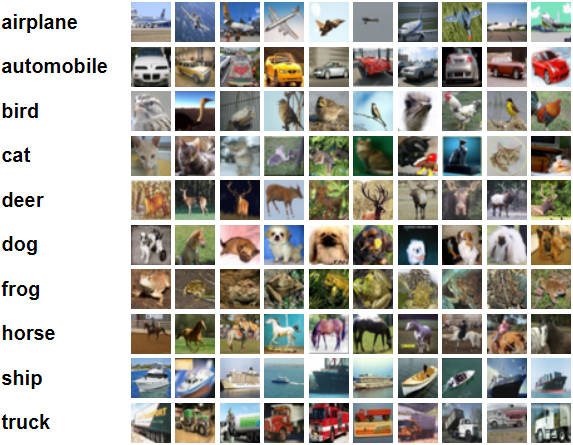
\includegraphics[width=0.6\textwidth]{./img/cifar-10.jpg}
	\caption{CIFAR-10 Dataset Example}
\end{figure}

\subsection{\textbf{Network Architecture}}

This part of the project is to build different neural network architectures and compare
their performance on the CIFAR-10 dataset. Networks we tried include: ResNet, PreActResNet,
WideResNet, ResNeXt, DenseNet, Dual Path Network, and Deep Layer Aggregation Network. By
training these networks with \textbf{fixed initial hyper-parameters and same training policy},
we will compare the optimal test accuracy of each network. After that, some ablation studies
will be conducted to investigate the effect of nets' \textbf{depth, width and cardinality}.

\subsubsection{\textbf{Brief Introduction}}

\textbf{ResNet} is a widely used network architecture for image classification. The
\textbf{residual block} proposed by He et al. efficiently solves the degradation problem
frequently occurred in deep networks, which is an \textbf{identity shortcut connection} that
skips one or more layers shown in the illustration below. Thanks to this kind of mapping,
the network can always backpropagate first-order information from one layer to another no
matter how deep it is, so as to address the problem of \textbf{vanishing/exploding gradient}.

\begin{figure}[H]
	\centering
	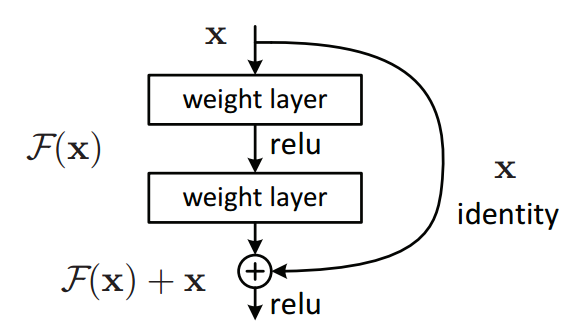
\includegraphics[width=0.5\textwidth]{./img/residual-block.png}
	\caption{Residual Block}
\end{figure}

\textbf{Pre-Activation ResNet} is a variant of ResNet that implements \textbf{pre-activation}
layers, in which case the shortcut connection stays \textbf{clean} because ReLU is applied in
conjunction with BatchNorm, thus the network no longer violates the identity mapping anymore.

\begin{figure}[H]
	\centering
	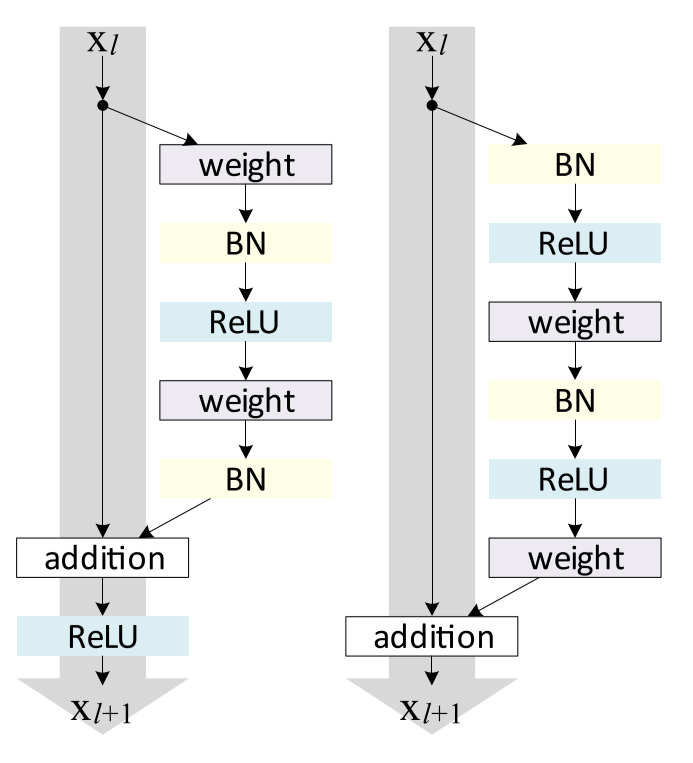
\includegraphics[width=0.5\textwidth]{./img/preact.png}
	\caption{\textbf{Left:} Residual Block. \textbf{Right:} Pre-Activation Block.}
\end{figure}

\textbf{Wide Residual Network} proposes that as the gradient flows through the network there
is nothing to force it to go through the residual block weights and thus it can avoid learning
during training, so it is possible that there is either only a few blocks that learn useful
representations, namely many blocks share very little information with small contribution to
the final goal. This problem is formulated as \textbf{diminishing feature reuse}. And as
widening the residual blocks, \textbf{dropout} should be inserted between convolutional layers
to \textbf{regularize training and prevent overfitting}.

\begin{figure}[H]
	\centering
	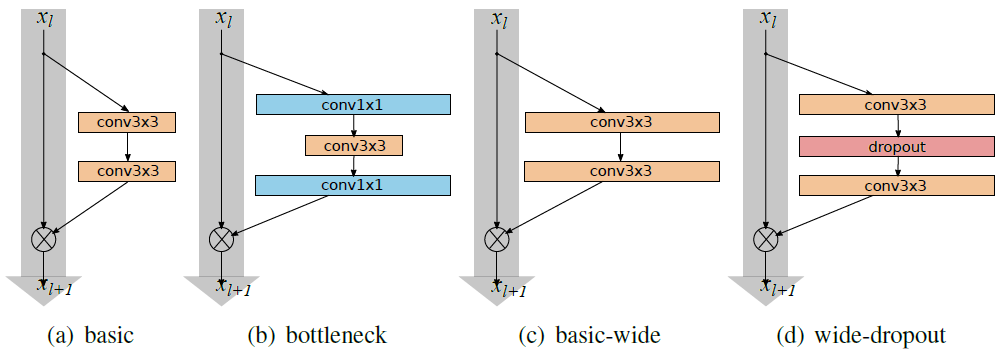
\includegraphics[width=0.9\textwidth]{./img/wrn.png}
	\caption{Wide Residual Block}
\end{figure}

\textbf{ResNeXt} repeats a building block that aggregates a set of transformations with the
same topology, indicating that \textbf{cardinality} (the size of the set of transformations)
is a concrete, measurable dimension that is of central importance, in addition to the
dimensions of width and depth.

Experiments have demonstrated that \textbf{increasing cardinality} is a more effective way
of gaining accuracy than going deeper or wider, especially when depth and width starts to
give diminishing returns for existing models. With roughly the same complexity, ResNeXt
can achieve higher accuracy than ResNet.

\begin{figure}[H]
	\centering
	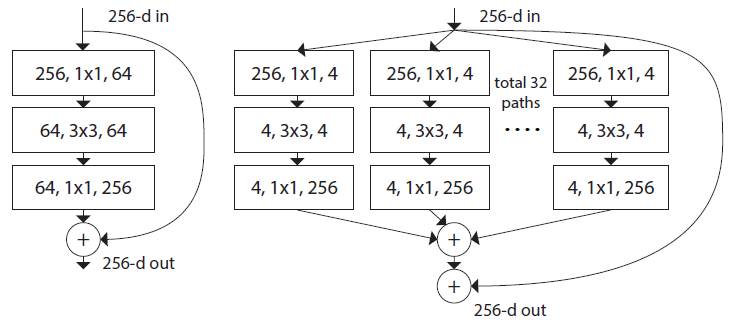
\includegraphics[width=0.8\textwidth]{./img/resnext.png}
	\caption{\textbf{Left:} Residual Block. \textbf{Right:} ResNeXt Block with cardinality = 32.}
\end{figure}

In \textbf{DenseNet}, each layer obtains additional inputs from all preceding layers and
passes on its own feature-maps to all subsequent layers. \textbf{Concatenation} is used.
Since each layer receives a \textbf{“collective knowledge”} from all preceding layers,
network can be \textbf{thin and compact}.

In this design, error signal can be easily propagated to earlier layers more which is is a
kind of \textbf{implicit deep supervision}, and with \textbf{smaller parameter size} comes
\textbf{more diversified features}.

\begin{figure}[H]
	\centering
	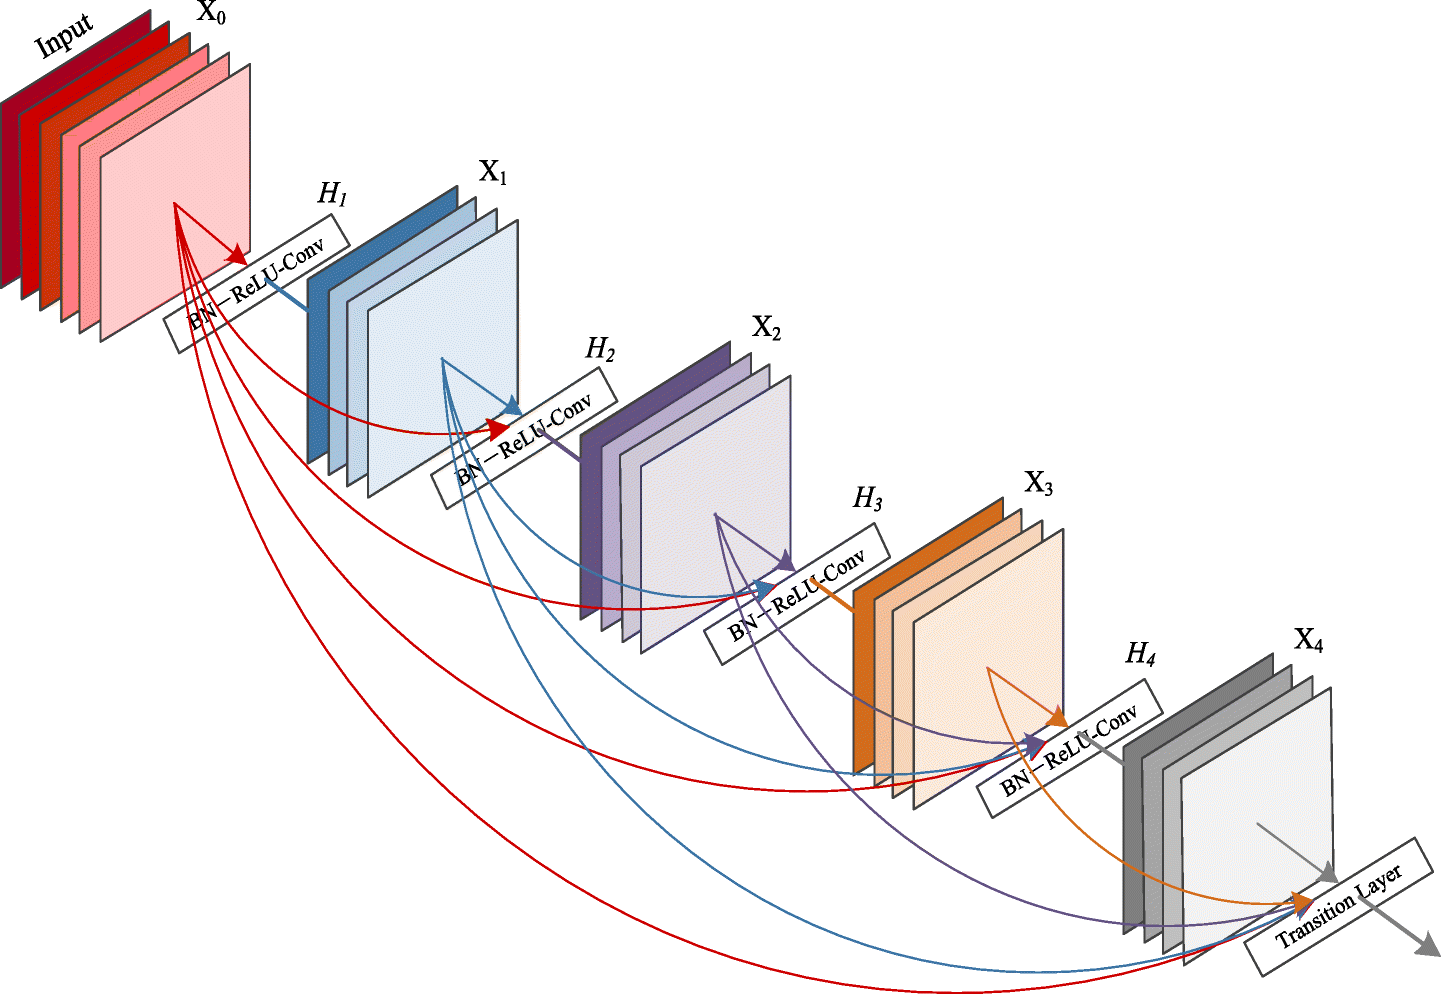
\includegraphics[width=0.7\textwidth]{./img/densenet.png}
	\caption{DenseNet Illustration}
\end{figure}

\textbf{Dual Path Network} is a convolutional neural network which presents a new topology
of connection paths internally. The intuition is that ResNets enables \textbf{feature re-usage}
while DenseNet enables \textbf{new feature exploration}, and both are important for learning
good representations. To enjoy the benefits from both path topologies, Dual Path Networks
\textbf{share common features} while maintaining the flexibility to \textbf{explore new features}
through dual path architectures.

\begin{figure}[H]
	\centering
	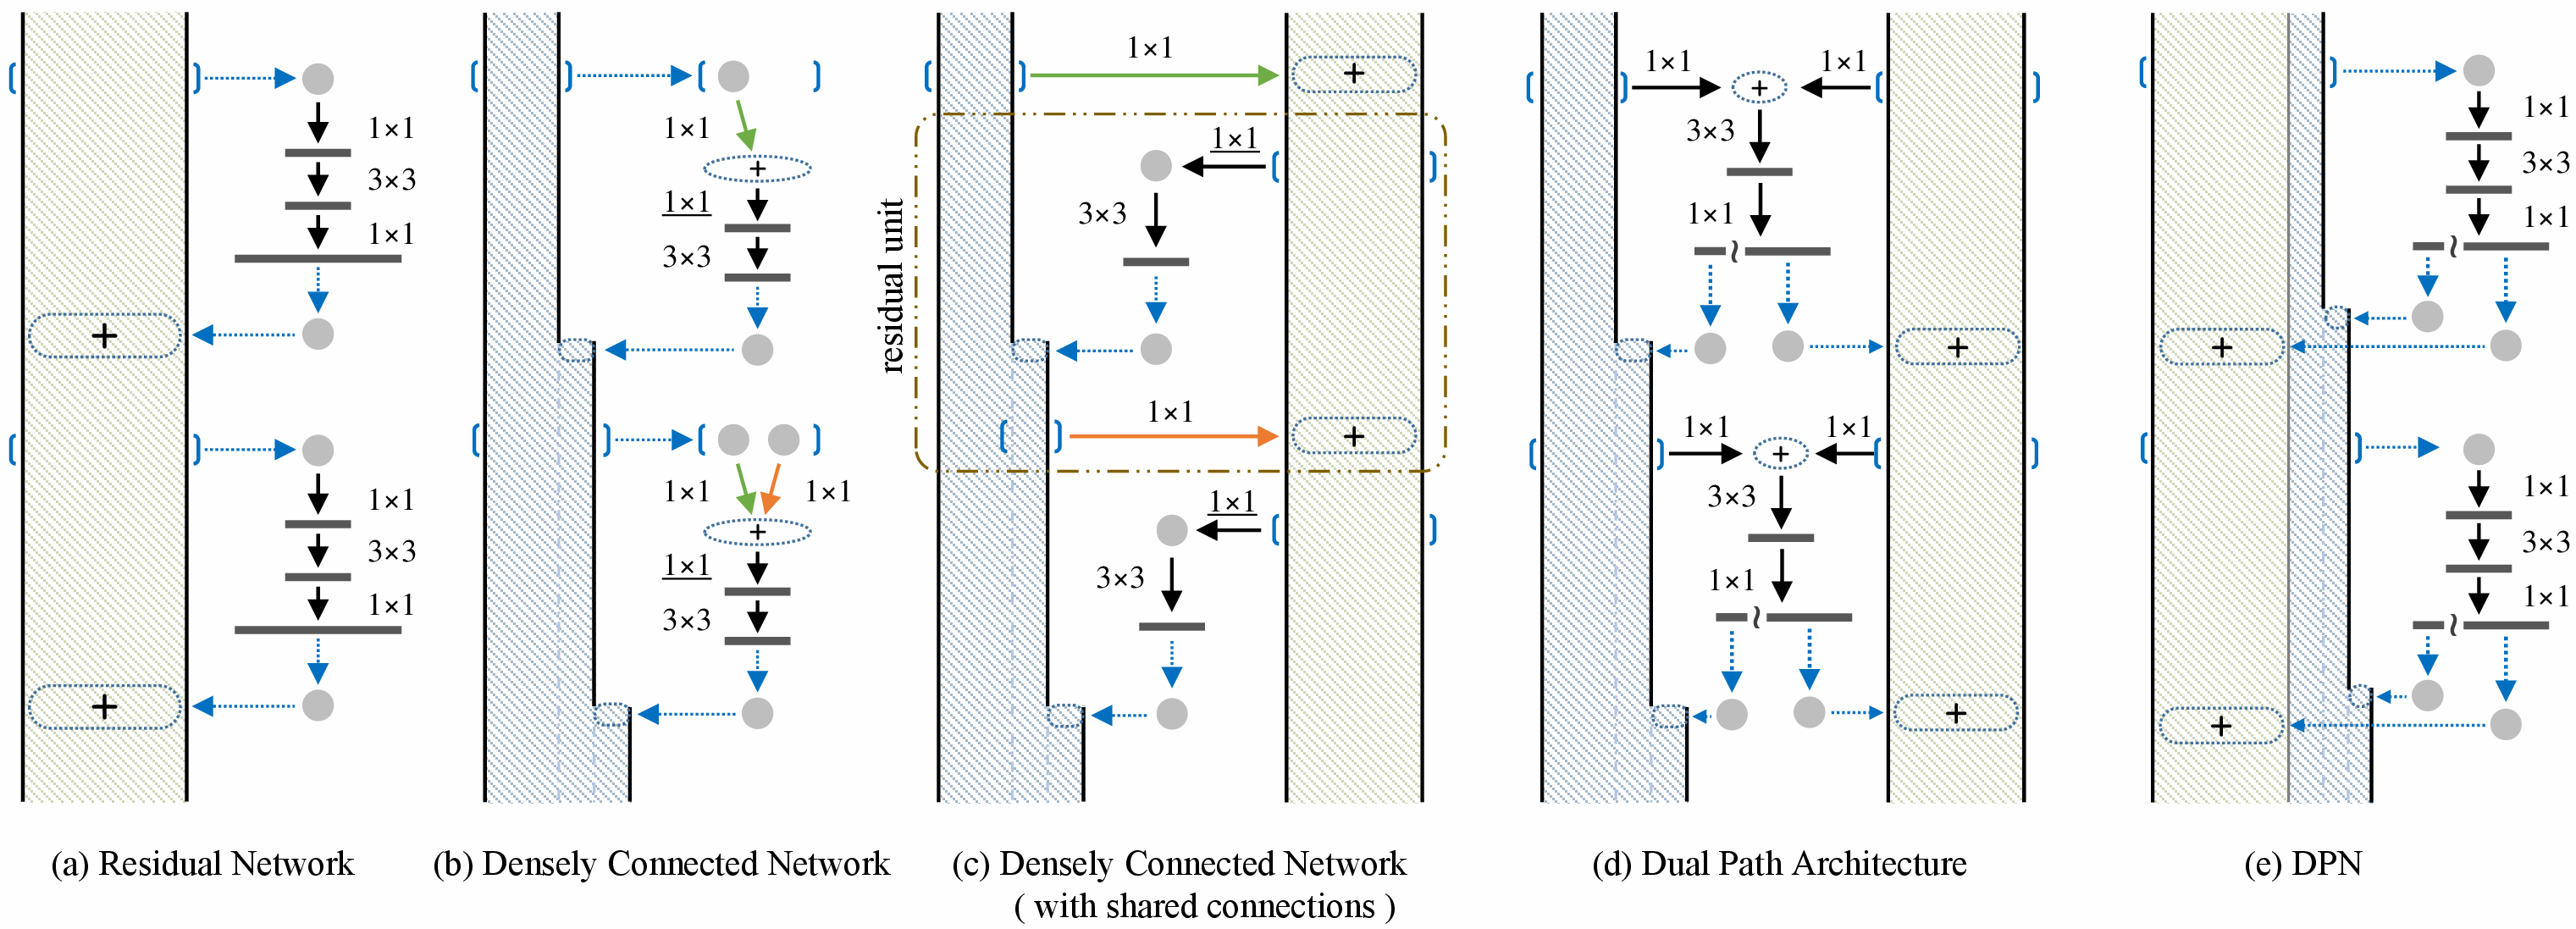
\includegraphics[width=1.0\textwidth]{./img/dpn.png}
	\caption{Dual Path Network}
\end{figure}

\textbf{Deep Layer Aggregation} learns to better extract the full spectrum of semantic and
spatial information from a network. \textbf{Iterative connections} join neighboring stages
to progressively deepen and spatially refine the representation. \textbf{Hierarchical connections}
cross stages with trees that span the spectrum of layers to better propagate features and
gradients. In nutshell, DLA makes no requirements of the internal structure of the blocks
and stages. DLA connects across stages with IDA, and within and across stages by HDA.

\begin{figure}[H]
	\centering
	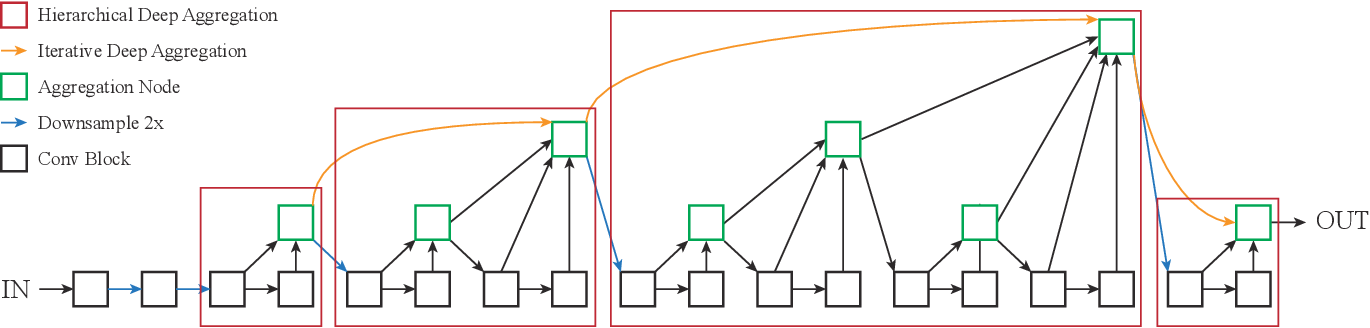
\includegraphics[width=1.0\textwidth]{./img/dla.png}
	\caption{Deep Layer Aggregation}
\end{figure}

\subsubsection{\textbf{Training Details}}

We train the models on the 50k training set and evaluate them on the 10k test set. The input
images are 32x32 \textbf{randomly cropped} from the \textbf{zero-padded} 40x40 images or
their \textbf{horizontally flipped versions}, and \textbf{normalization} is performed in the
preprocessing step as well. \textbf{No other data augmentation is applied}.

As for the optimizer, we simply use \textbf{SGD} with a mini-batch size of \textbf{128}, the
momentum and weight decay are set to \textbf{0.9} and \textbf{5e-4} respectively. Furthermore,
the learning rate of which is starting at \textbf{0.1} and decreasing by a factor of
\textbf{0.5} when the test error plateaus, and the models are trained for \textbf{200} epochs.

For more code details, please refer to the attached \textbf{main.py} file.

\subsubsection{\textbf{General Results}}

We conduct experiments on CIFAR-10 using the models mentioned above, and results are shown in
the following table (ps. number of parameters may be different from original paper due to the
manual implementation for CIFAR-10 dataset).

\begin{table}[H]
	\begin{center}
		\begin{tabular}{ccc}
			\toprule
			architecture             & $\#$params & error         \\
			\midrule
			ResNet-18                & 11.17M     & 4.89          \\
			PreActResNet-18          & 11.17M     & 5.12          \\
			WRN-28-10                & 36.49M     & \textbf{4.27} \\
			ResNeXt-29, 32$\times$4d & 4.77M      & 4.85          \\
			DenseNet-121             & 6.96M      & 4.78          \\
			DPN-26                   & 11.57M     & 5.21          \\
			DLA                      & 16.29M     & 5.02          \\
			\bottomrule
		\end{tabular}
		\caption{Top-1 error($\%$) and model size on CIFAR-10}
	\end{center}
\end{table}

Take ResNet-18 as the benchmark, we can observe that WRN-28-10, ResNeXt-29 and DenseNet-121
achieve lower top-1 error while which is to our surprise, PreActResNet-18, DPN-26 and DLA
go even worse.

The reason of performance degradation on the latter two might be that their model complexity
is far greater than the CIFAR-10 classification task requires, therefore, 200 epochs is not
enough for convergence.

For instance, the training process of ResNet-18 is visualized in the figure below.

\begin{figure}[H]
	\centering
	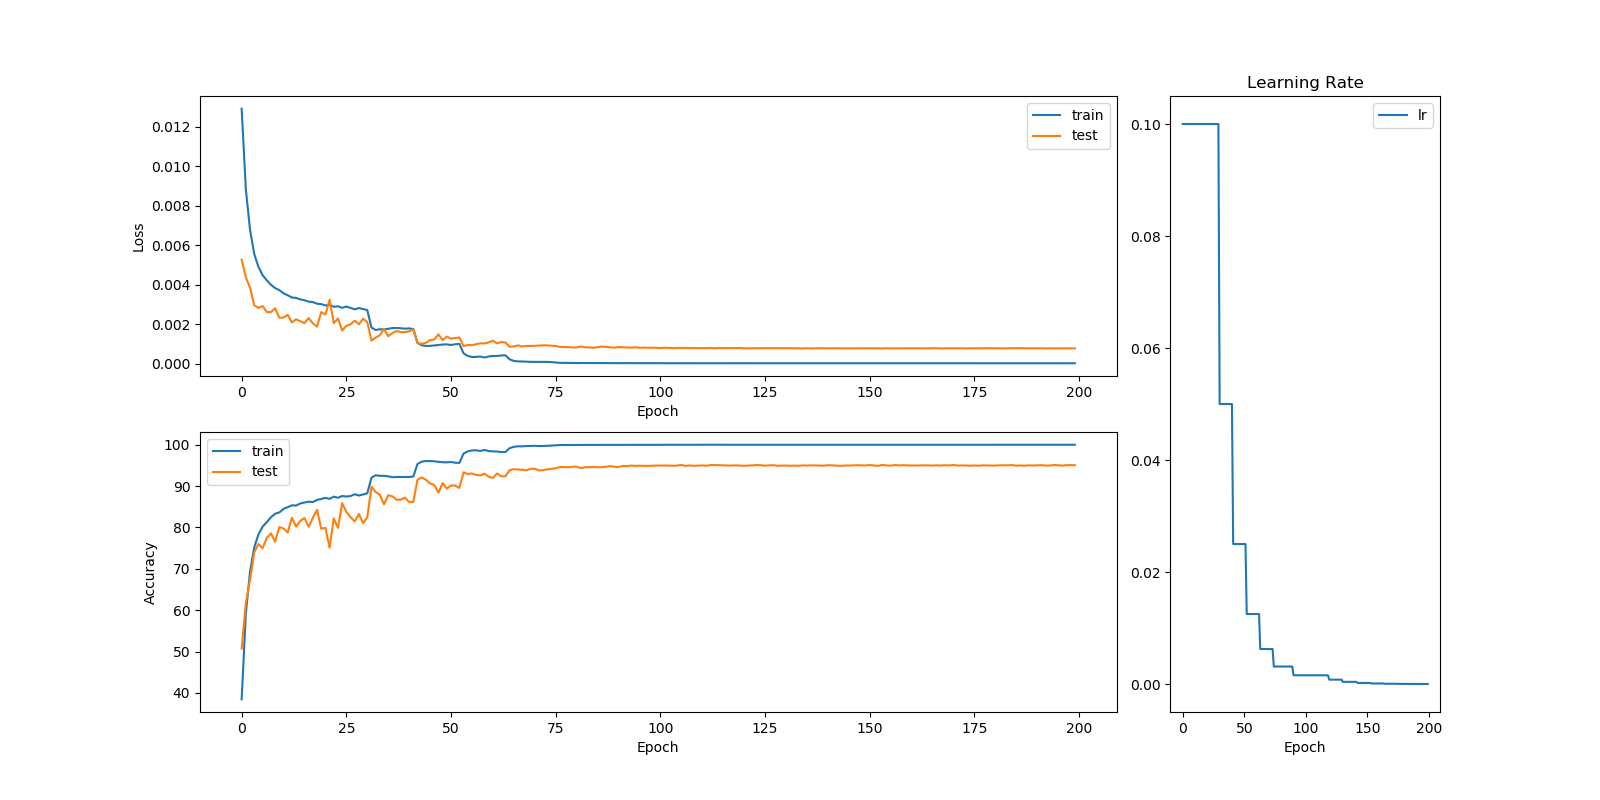
\includegraphics[width=1.0\textwidth]{./img/resnet-18.png}
	\caption{Training process of ResNet-18}
\end{figure}

\subsubsection{\textbf{Ablation Experiments}}

We conduct ablation experiments on CIFAR-10 classification task in order to investigate
the effect of network hyper-parameters on performance, like
\textbf{depth, width and cardinality}. The results are shown in the following table.

\begin{table}[H]
	\centering
	\begin{tabular}{cccc}
		\toprule
		architecture & setting & $\#$params & error         \\
		\midrule
		ResNet-18    & 1x64d   & 11.17M     & \textbf{4.89} \\
		ResNet-50    & 1x64d   & 23.52M     & 5.37          \\
		\midrule
		ResNeXt-29   & 2x32d   & 2.30M      & 5.78          \\
		ResNeXt-29   & 2x64d   & 9.13M      & \textbf{4.54} \\
		\midrule
		ResNeXt-29   & 2x64d   & 9.13M      & 4.54          \\
		ResNeXt-29   & 8x64d   & 89.60M     & \textbf{4.19} \\
		\midrule
		ResNet-50    & 1x64d   & 23.52M     & 5.37          \\
		ResNeXt-50   & 2x40d   & 17.30M     & 5.33          \\
		ResNeXt-50   & 8x14d   & 20.86M     & 4.80          \\
		ResNeXt-50   & 32x4d   & 22.98M     & \textbf{4.54} \\
		\bottomrule
	\end{tabular}
	\caption{Ablation experiments on CIFAR-10}
	\label{tab:ablation}
\end{table}

\textbf{Depth.} We envaluate effect of depth via ResNet-18 and ResNet-50, it can be seen
that the former gains higher accuracy under 200 epochs while maintaining the other same
training conditions like optimizer or learning rate scheduler. Therefore, we may come up
with the conclusion that \textbf{it's not always a good idea to just use deeper network},
not only because of the model complexity and converging time, but also for some possibly
redundant layers.

\textbf{Width.} The second part is about width, which refers to the number of channels in
a layer. Experiment indicates that the higher the width, the lower the top-1 error. It
seems that with parameters of this magnitude, a \textbf{wider} network can always achieve
better accuracy, for the convergence speed does not slow down much.

\textbf{Cardinality.} Next we investigate increasing complexity by increasing cardinality.
We roughly compare the performance of ResNeXt-29 with fixed width 64 but varying cardinality
2 and 8. The latter achieves higher accuracy up to \textbf{95.81$\%$}, which is the highest
so far. However, the training process is \textbf{quite slow} due to the large number of
parameters involved (\textbf{89.60M}).

\textbf{Cardinality vs. Width.} Last but not least, we evaluate the trade-off between
cardinality and width, under preserved complexity as listed in Table \ref{tab:ablation}.
Comparing with ResNet-50, the ResNeXt-50 32x4d has a test error of 4.54$\%$, which is
\textbf{0.83$\%$} lower than the ResNet baseline's 5.37$\%$. With cardinality increasing
from 1 to 32 while keeping approximately the same complexity, the test error rate keeps
reducing. Furthermore, the 32x4d version also has a much lower training error than the
counterpart to the same period, suggesting that the gains are
\textbf{not from regularization but from stronger representations},
and we may draw the preliminary conclusion that
\textbf{increasing cardianlity shows better results than going wider}.

\subsection{\textbf{Other Inquries}}

\subsubsection{\textbf{Training Details}}

For simplicity, \textbf{ResNet-18} with \textbf{ReLU} is used as the benchmark model. Same
image preprocessing techniques as in the previous section are applied. As for loss function,
we choose \textbf{CrossEntropy} implemented in PyTorch, .and \textbf{Adam} optimizer with
initial learning rate 0.001 and reduce-on-plateau is adopted. One more thing, different from
the preceding configuration, max training epoch is set to \textbf{50}.

\subsubsection{\textbf{Activation Layer}}

Replace all the activation layers with \textbf{Sigmoid, Leaky ReLU, ELU or GELU}. Here are
the results.

\begin{figure}[H]
	\centering
	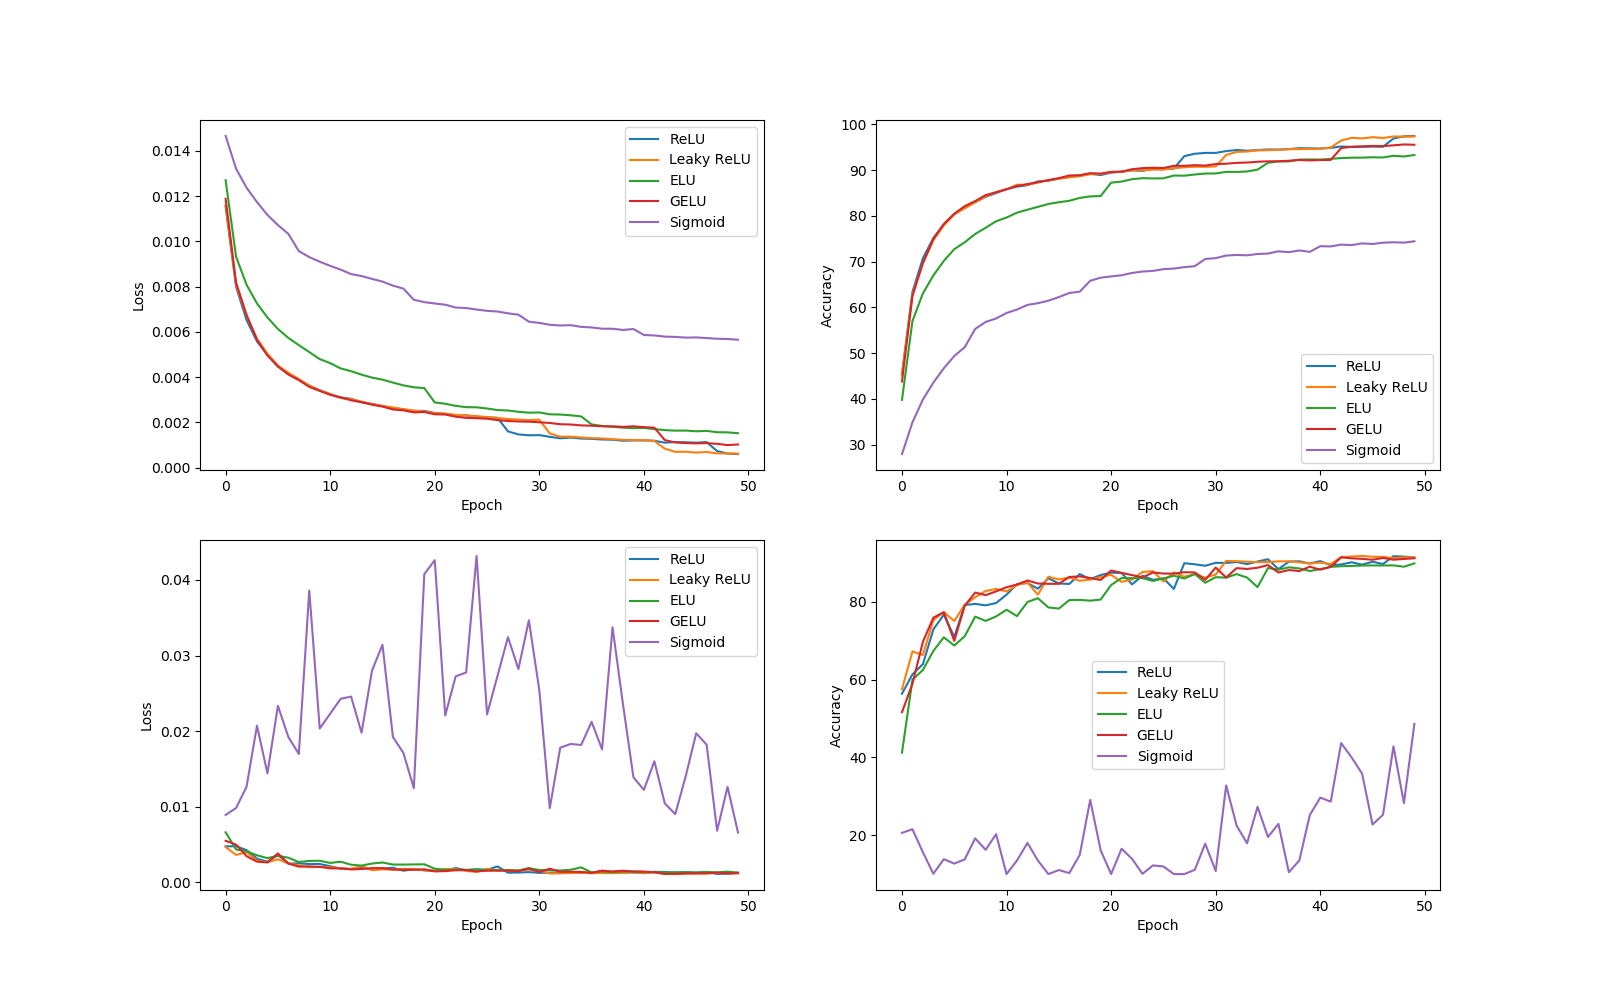
\includegraphics[width=1.0\textwidth]{./img/activation.png}
	\caption{Different activation layers (\textbf{Upper:} Training. \textbf{Lower:} Test.)}
\end{figure}

Sigmoid activation layer looks out of place, while the others are united in convergent
behavior. Among ReLU family, Leaky ReLU is the relatively fastest one and ELU is on the
contrary, and from test accuracy perspective, GELU is the most \textbf{stable} one with
visually minimum volatility.

For more code details, please refer to the attached \textbf{main\_activation.py} file.

\subsubsection{\textbf{Loss Function}}

We attempt some other criterion like \textbf{BCELoss, MSELoss, HuberLoss} to see the effect
of the loss function. Here presented are the results.

\begin{figure}[H]
	\centering
	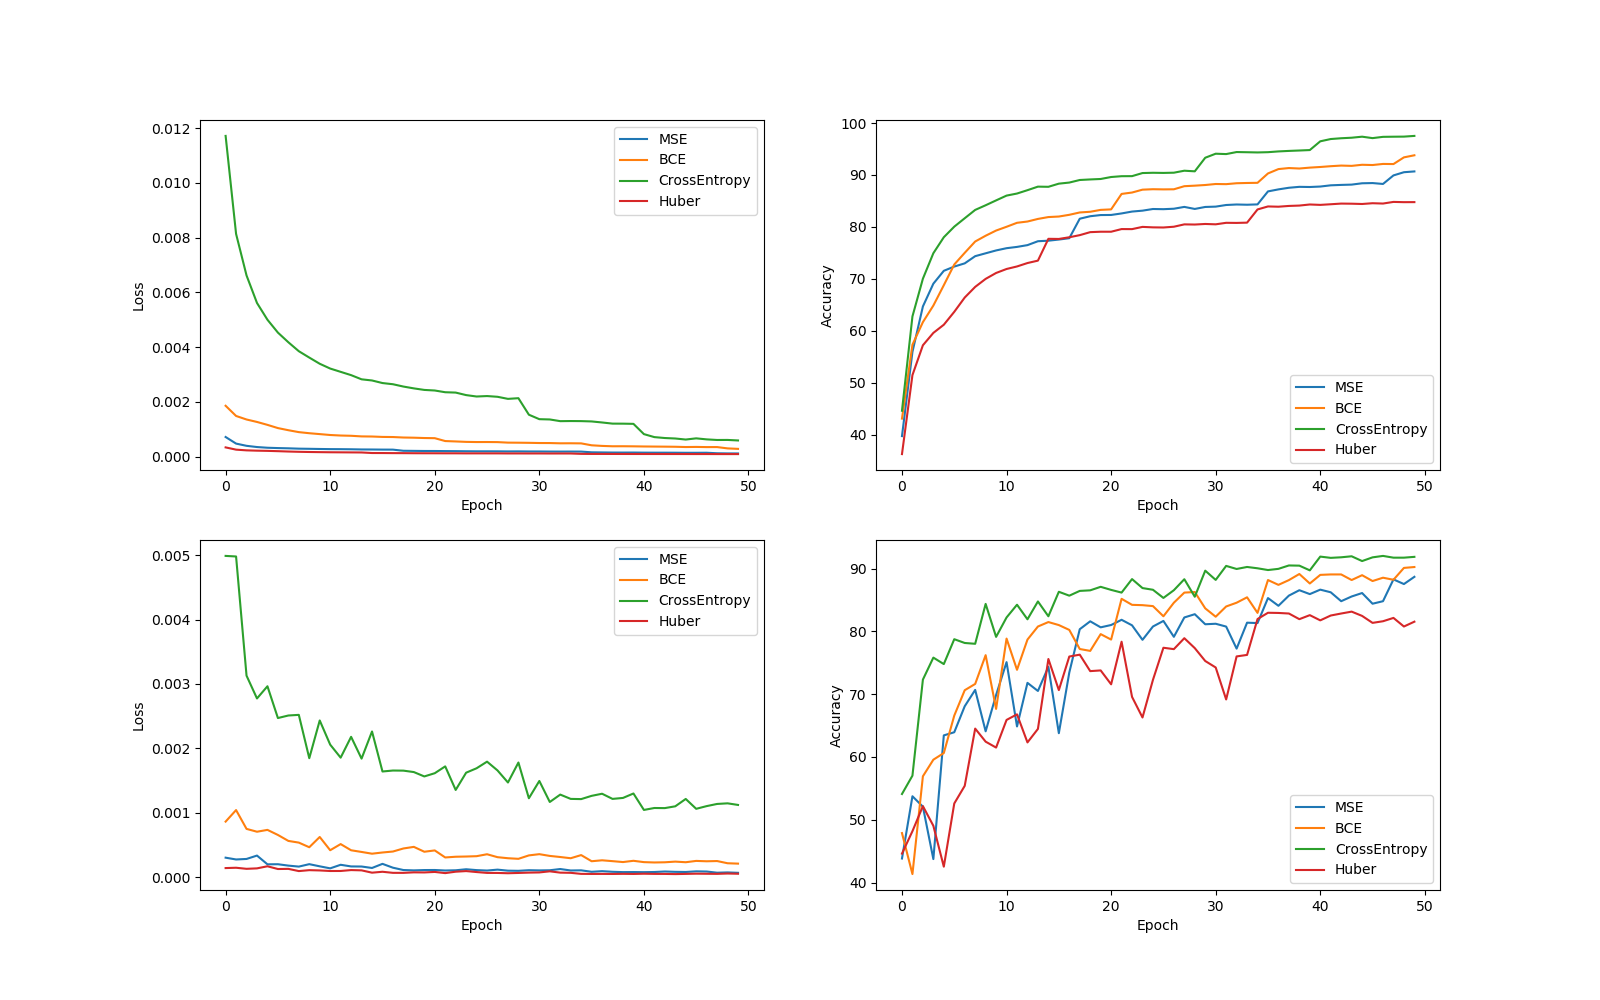
\includegraphics[width=1.0\textwidth]{./img/criterion.png}
	\caption{Different Loss Functions (\textbf{Upper:} Training. \textbf{Lower:} Test.)}
\end{figure}

From the log image, phenomenon can be observed that the stratification is quite significant
in each subfigure, manifesting the classification capability ranking should be: CrossEntropy
$>$ BCELoss $>$ MSELoss $>$ HuberLoss.

For more code details, please refer to the attached \textbf{main\_criterion.py} file.

\subsubsection{\textbf{Optimizer}}

This part we try different optimizers, including \textbf{SGD, Adagrad, Adadelta, Adam}, and
results are shown in the following figure.

\begin{figure}[H]
	\centering
	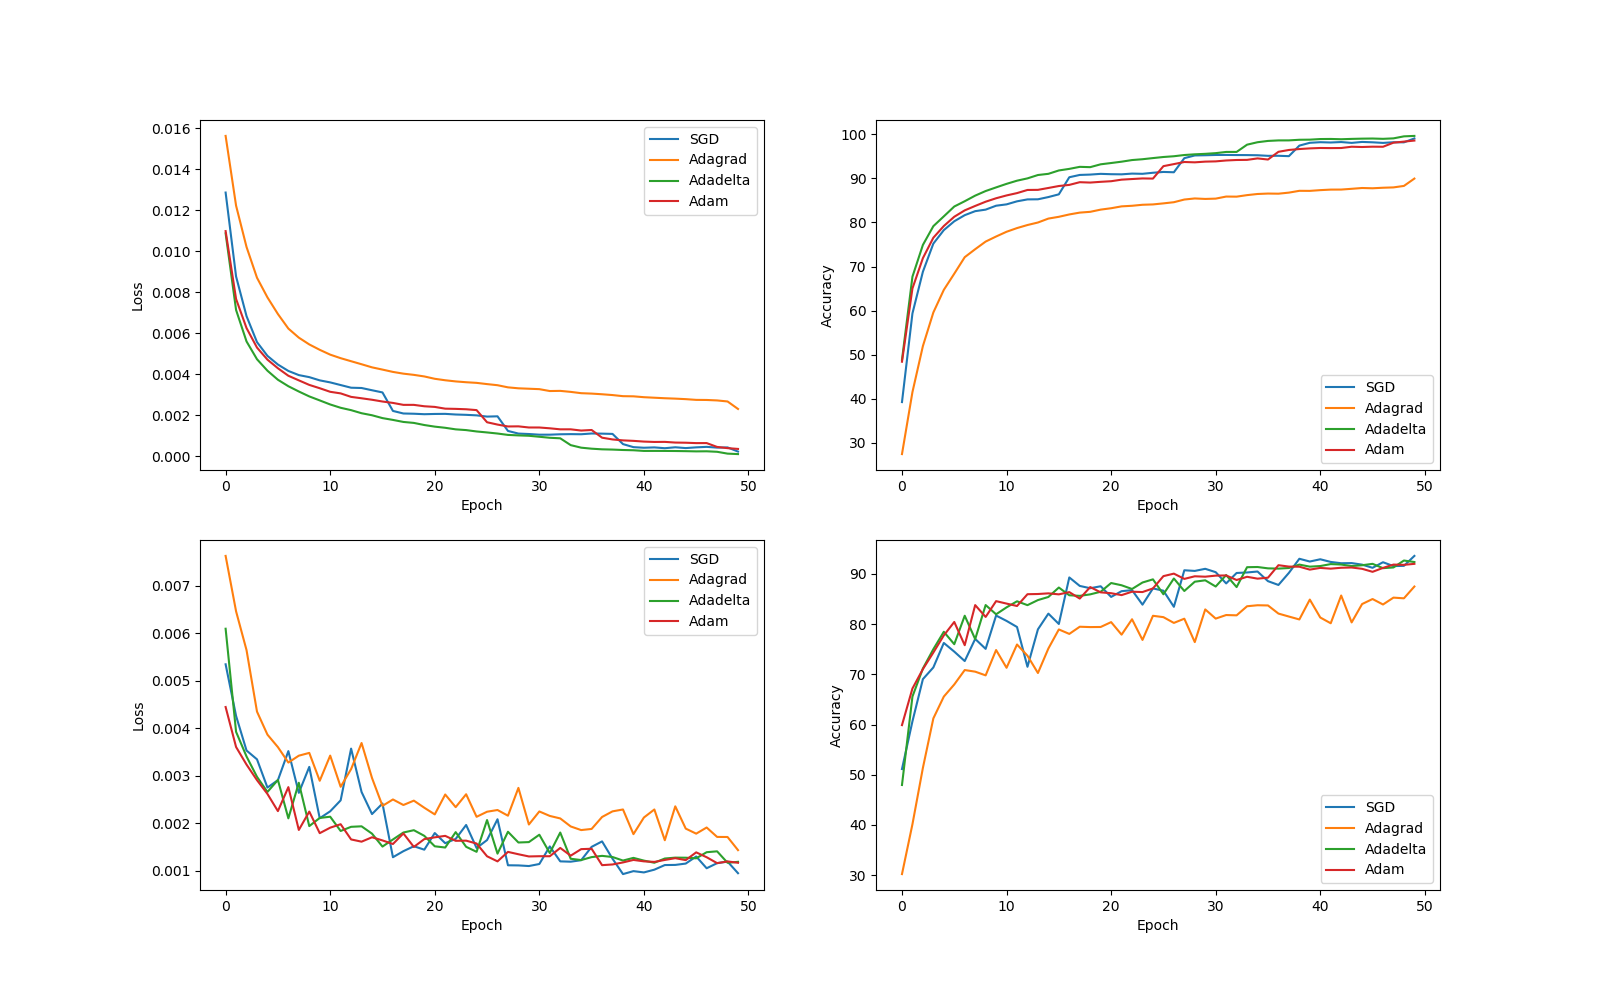
\includegraphics[width=1.0\textwidth]{./img/optimizer.png}
	\caption{Different Optimizers (\textbf{Upper:} Training. \textbf{Lower:} Test.)}
\end{figure}

Adagrad performs worse in terms of every subfigure, while others are on the same level.

\subsection{\textbf{Network Interpretation}}

Ramprasaath R. Selvaraju et al. proposed a technique for producing "visual explanations"
for decisions from a large class of \textbf{CNN-based models}, making them more transparent.
Their approach - \textbf{Gradient-weighted Class Activation Mapping (Grad-CAM)}, uses the
gradients of any target concept, flowing into the \textbf{final convolutional layer} to
produce a coarse localization map highlighting important regions in the image for predicting
the concept.

The following figure shows the results of Grad-CAM for ResNet-18.

\begin{figure}[H]
	\centering
	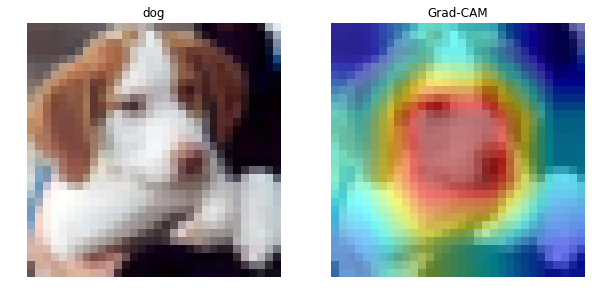
\includegraphics[width=0.6\textwidth]{./img/grad-cam.png}
	\caption{Grad-CAM for ResNet-18}
\end{figure}

\subsection{\textbf{Best Model}}

Our best model is \textbf{WideResNet-28-10} with extra \textbf{Cutout} augmentation, other
preprocessings are just as usual. The test accuracy achieves \textbf{96.65$\%$} in 200
epochs, and the powerful effect of Cutout augmentation reflects in the training process
saliently compared with any other techniques.

\begin{figure}[H]
	\centering
	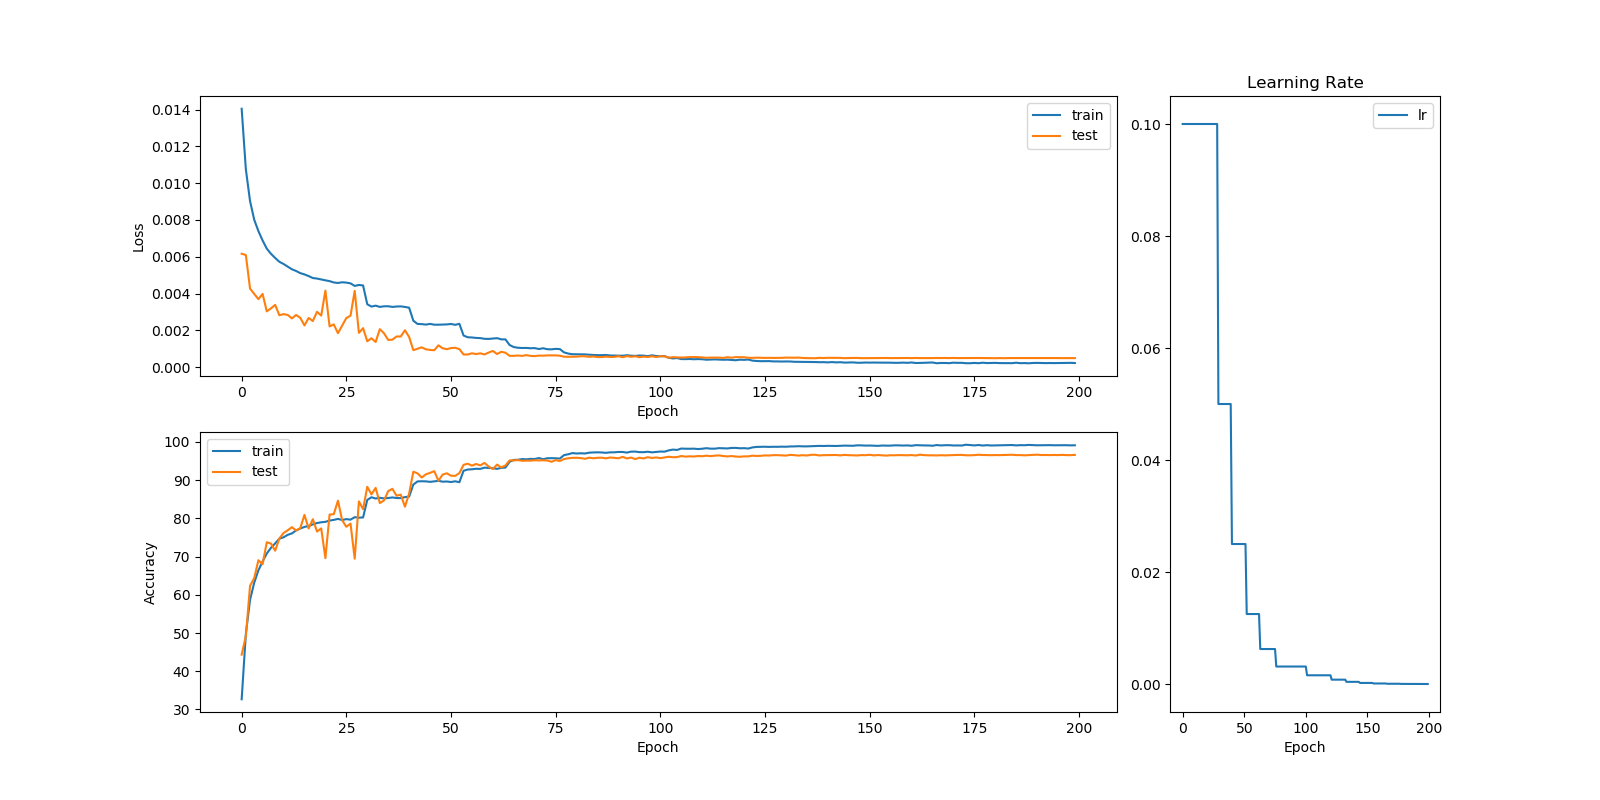
\includegraphics[width=1.0\textwidth]{./img/best.png}
	\caption{WRN-28-10 with \textbf{Cutout}}
\end{figure}

\bigskip

%------------------------------------------------

\section{\textbf{Batch Normalization}}

Batch Normalization aims to \textbf{reduce internal covariate shift}, and in doing so aims
to accelerate the training of deep neural nets. It accomplishes this via a normalization
step that fixes the means and variances of layer inputs. Batch Normalization also has a
beneficial effect on the gradient flow through the network, by reducing the dependence of
gradients on \textbf{the scale of the parameters or of their initial values}. This allows
for \textbf{use of much higher learning rates without the risk of divergence}. Furthermore,
batch normalization regularizes the model and reduces the need for Dropout.

The implementation of Batch Normalization for a minibatch $\mathcal{B}$ is as follows:

$$
	\begin{gathered}
		\mu_{\mathcal{B}}=\frac{1}{m} \sum_{i=1}^{m} x_{i} \\
		\sigma_{\mathcal{B}}^{2}=\frac{1}{m} \sum_{i=1}^{m}\left(x_{i}-\mu_{B}\right)^{2} \\
		\hat{x}_{i}=\frac{x_{i}-\mu_{\mathcal{B}}}{\sqrt{\sigma_{\mathcal{B}}^{2}+\epsilon}} \\
		y_{i}=\gamma \hat{x}_{i}+\beta=\mathrm{BN}_{\gamma, \beta}\left(x_{i}\right)
	\end{gathered}
$$

Where $\gamma$ and $\beta$ are \textbf{learnable parameters}, $\epsilon$ is a small constant
to avoid division by zero.

Recent research results show that BN reparametrizes the underlying optimization problem to
make its landscape significantly more smooth. So along this line, we are going to measure:

\begin{enumerate}
	\item Loss landscape or variation of the value of the loss.
	\item Gradient predictiveness or the change of the loss gradient.
	\item Maximum difference in gradient over the distance.
\end{enumerate}

\subsection{\textbf{Loss Landscape}}

By setting the learning rate to 2e-3, 1e-3, 5e-4 and 1e-4 and training each for 20 epochs,
the fill-between plot of the loss landscape can be shown in the following figure. This is
a loss-step plot, since the batch size is 128, there will be nearly 8,000 steps in total.

\begin{figure}[H]
	\centering
	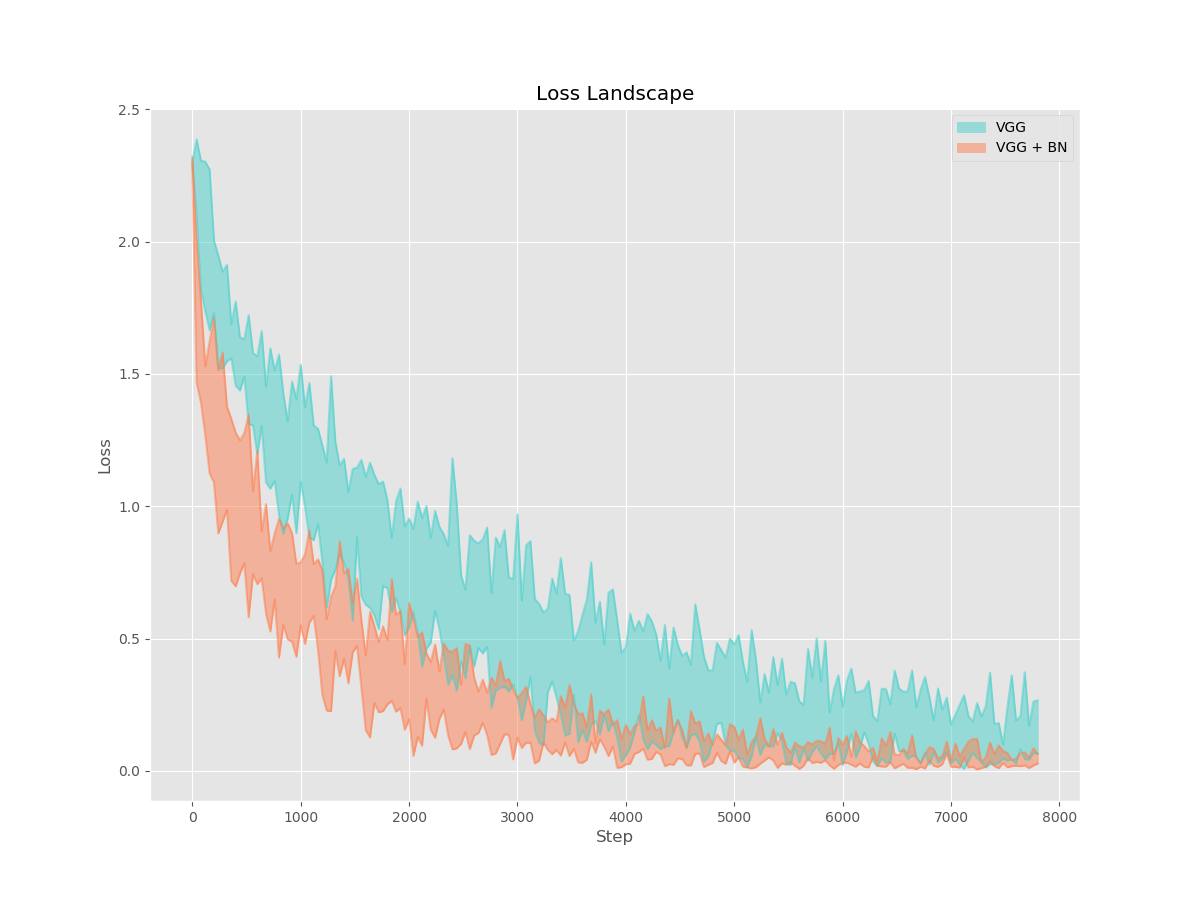
\includegraphics[width=0.9\textwidth]{./img/loss-lands.png}
	\caption{Loss landscape for VGG-A with and without BatchNorm}
\end{figure}

From figure above, we can easily draw the conclusion that BatchNorm really helps to reduce
the loss variance and thus boost the training speed.

\subsection{\textbf{Gradient Predictiveness}}

Keeping the same hyper-parameters, we intend to record the change of gradient in last linear
layer where the metric chosen is the \textbf{L2 norm} of the gradient difference. Results
are presented in the following figure.

\begin{figure}[H]
	\centering
	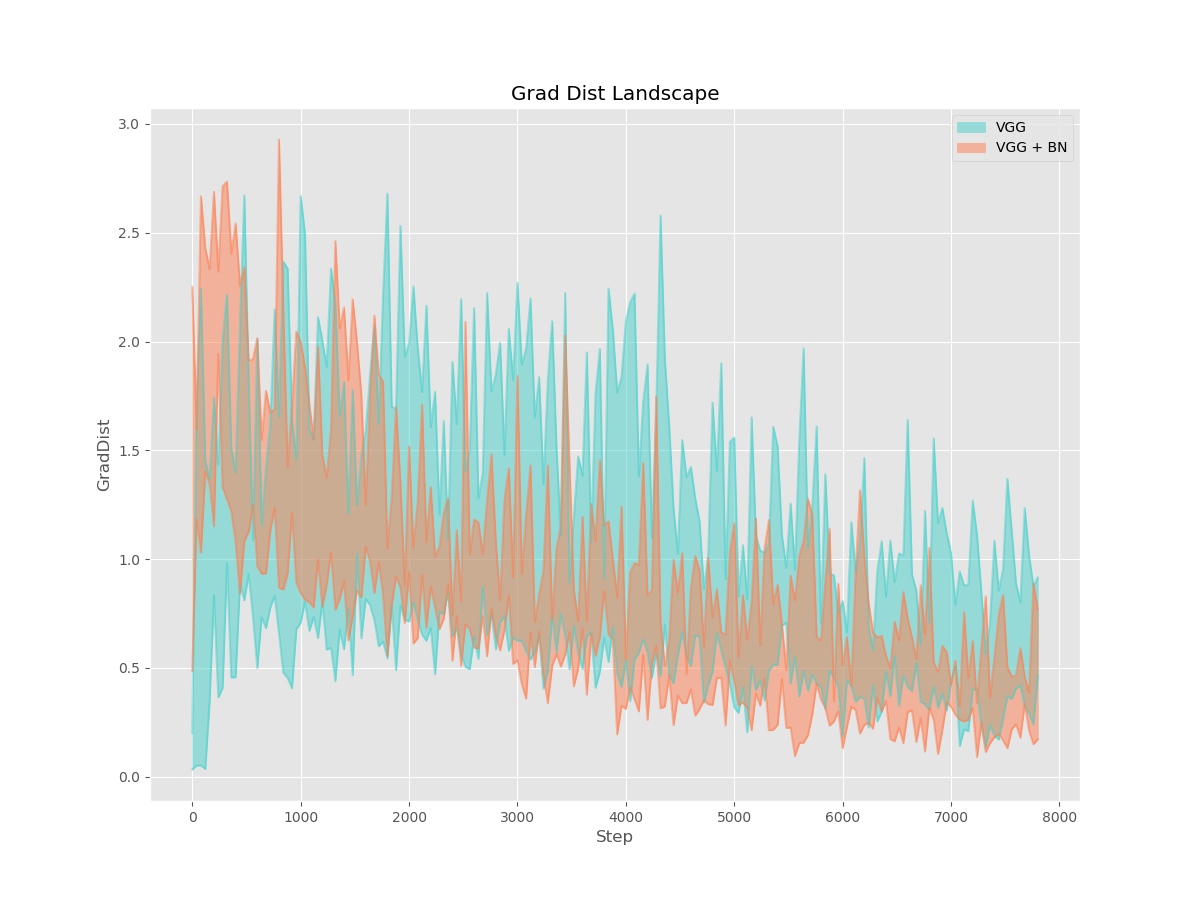
\includegraphics[width=0.9\textwidth]{./img/grad-lands.png}
	\caption{Gradient predictiveness for VGG-A with and without BatchNorm}
\end{figure}

As for the general trend of the gradient predictiveness, we can find that VGG with BatchNorm
is batter and more stable than VGG without BatchNorm because of the lower L2 distance and
more smooth volatility.

\subsection{\textbf{Beta Smoothness}}

Recall that $f$ is $\beta$-smooth if its gradient is $\beta$-Lipschitz. It is worth noting
that, due to the existence of non-linearities, one should not expect the $\beta$-smoothness
to be bounded in an absolute, global sense.

$$
	\left\|\nabla f\left(w_{t+1}\right)-\nabla f\left(w_{t}\right)\right\| \leq \beta_{t} \left\|w_{t+1}-w_{t}\right\|
$$

And we know that the update of $w$ provided by SGD from $t$ to $t+1$ is

$$
	w_{t+1}=w_{t}-lr*\nabla f\left(w_{t}\right)
$$

Thus we can derive $\beta$ from the following formula:

$$
	\beta_{t} = \max \frac{\left\|\nabla f\left(w_{t+1}\right)-\nabla f\left(w_{t}\right)\right\|}{lr*\left\|\nabla f\left(w_{t}\right)\right\|}
$$

Or just use

$$
	\beta_{t} = \max \frac{\left\|\nabla f\left(w_{t+1}\right)-\nabla f\left(w_{t}\right)\right\|}{\left\|w_{t+1}-w_{t}\right\|}
$$

for Adam optimizer.

\begin{figure}[H]
	\centering
	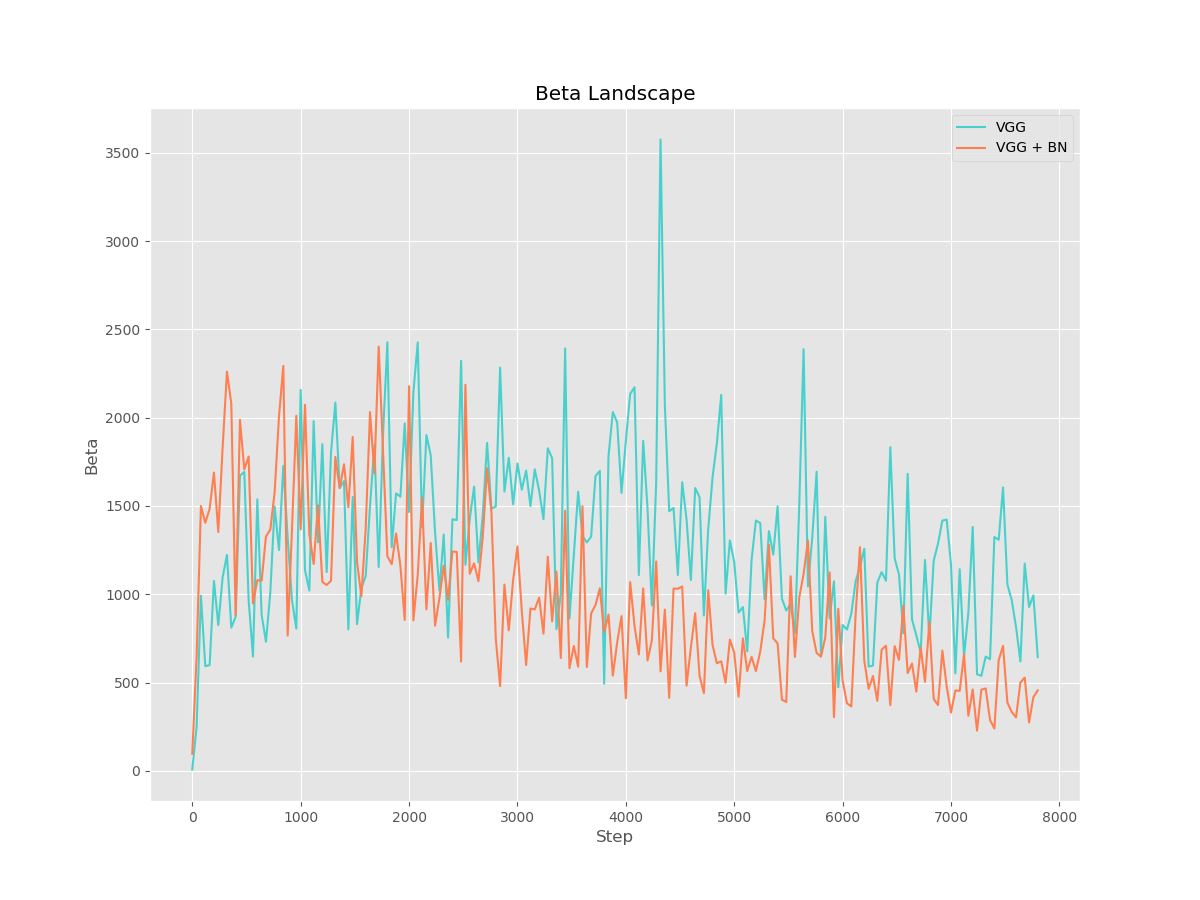
\includegraphics[width=0.85\textwidth]{./img/beta-smooth.png}
	\caption{Beta Smoothness for VGG-A with and without BatchNorm}
\end{figure}

\bigskip

%------------------------------------------------

\section{\textbf{DessiLBI}}

The great success of deep neural networks is built upon their over-parameterization, which
smooths the optimization landscape without degrading the generalization ability. Despite
the benefits of over-parameterization, a huge amount of parameters makes deep networks
cumbersome in daily life applications. On the other hand, training neural networks without
over-parameterization faces many practical problems, e.g., being trapped in local optimal.
Though techniques such as pruning and distillation are developed, they are expensive in
fully training a dense network as backward selection methods, and there is still a void
on systematically exploring forward selection methods for learning structural sparsity in
deep networks. To fill in this gap, this paper proposes a new approach based on differential
inclusions of inverse scale spaces. Specifically, our method can generate a family of
models from simple to complex ones along the dynamics via coupling a pair of parameters,
such that over-parameterized deep models and their structural sparsity can be explored
simultaneously. This kind of differential inclusion scheme has a simple discretization,
dubbed Deep structure splitting Linearized Bregman Iteration (DessiLBI), whose global
convergence in learning deep networks could be established under the Kurdyka-Łojasiewicz
framework.

\subsection{\textbf{LeNet on MNIST}}

Applying SLBI and SGD for LeNet on MNIST dataset respectively, we can compare the performance
of the two optimizers. The results are shown in the following figure.

\begin{figure}[H]
	\begin{minipage}[t]{0.48\textwidth}
		\centering
		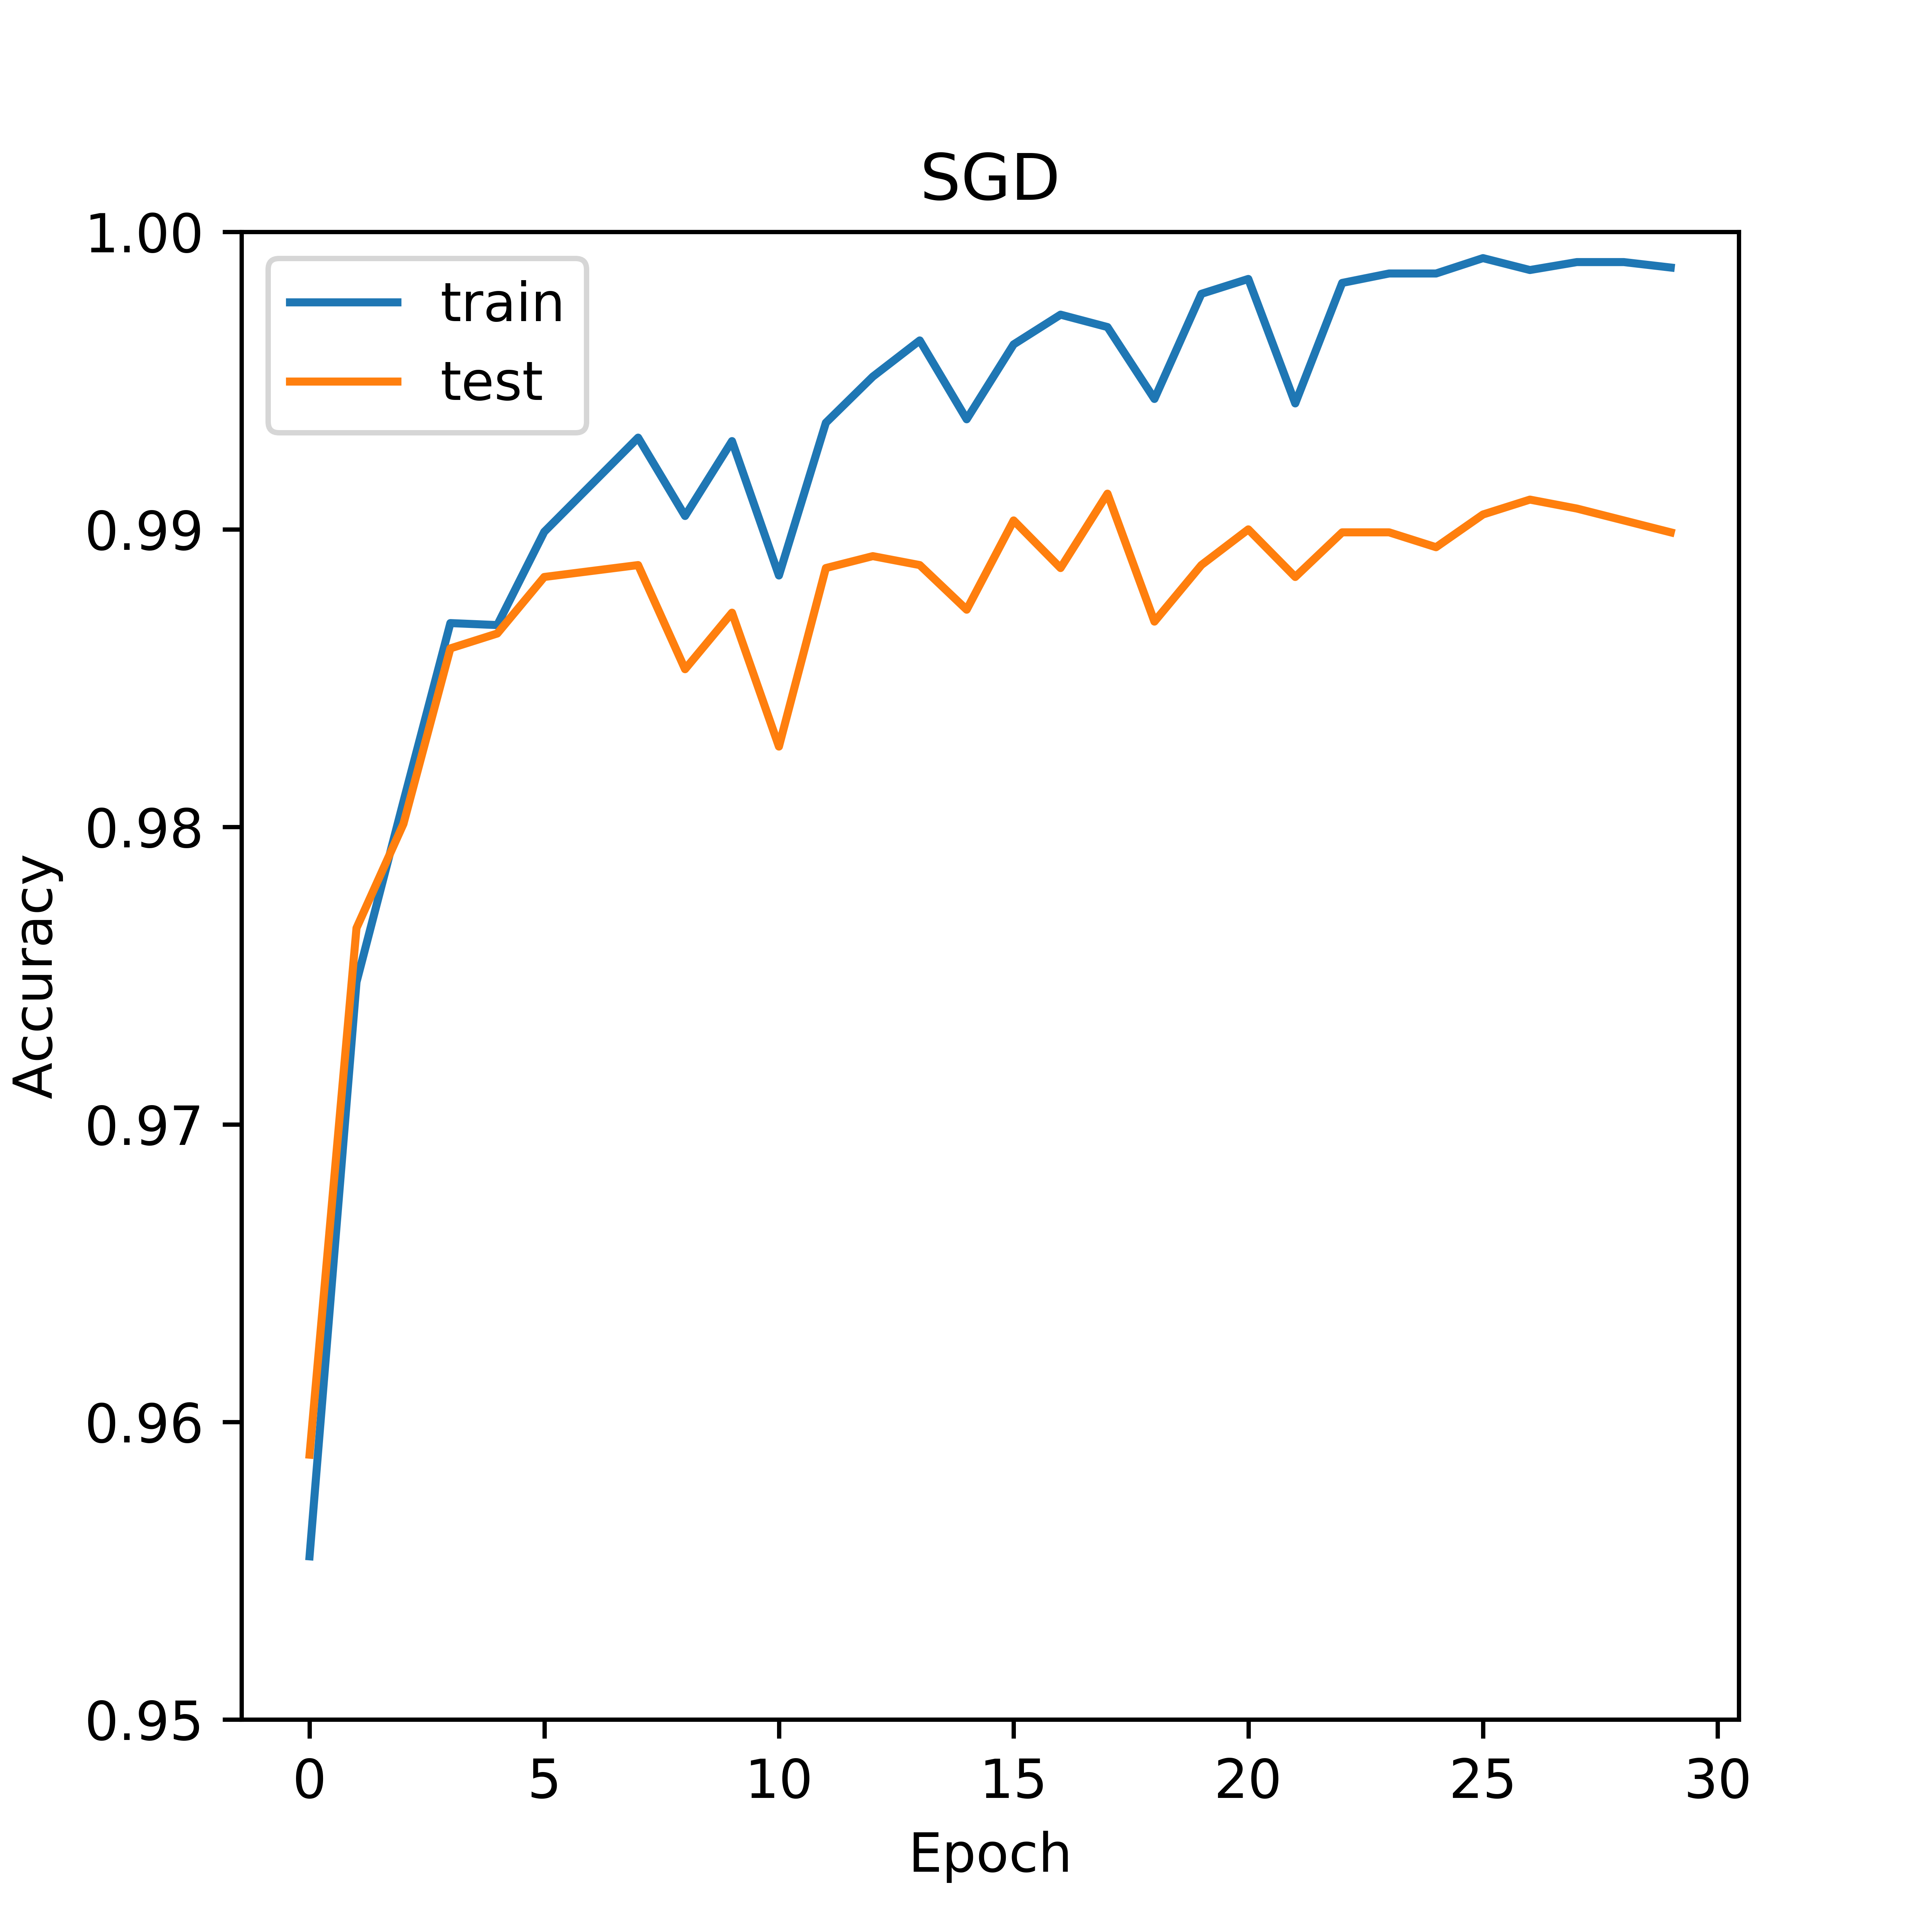
\includegraphics[width=2.5in]{./img/train-sgd.png}
	\end{minipage}
	\begin{minipage}[t]{0.48\textwidth}
		\centering
		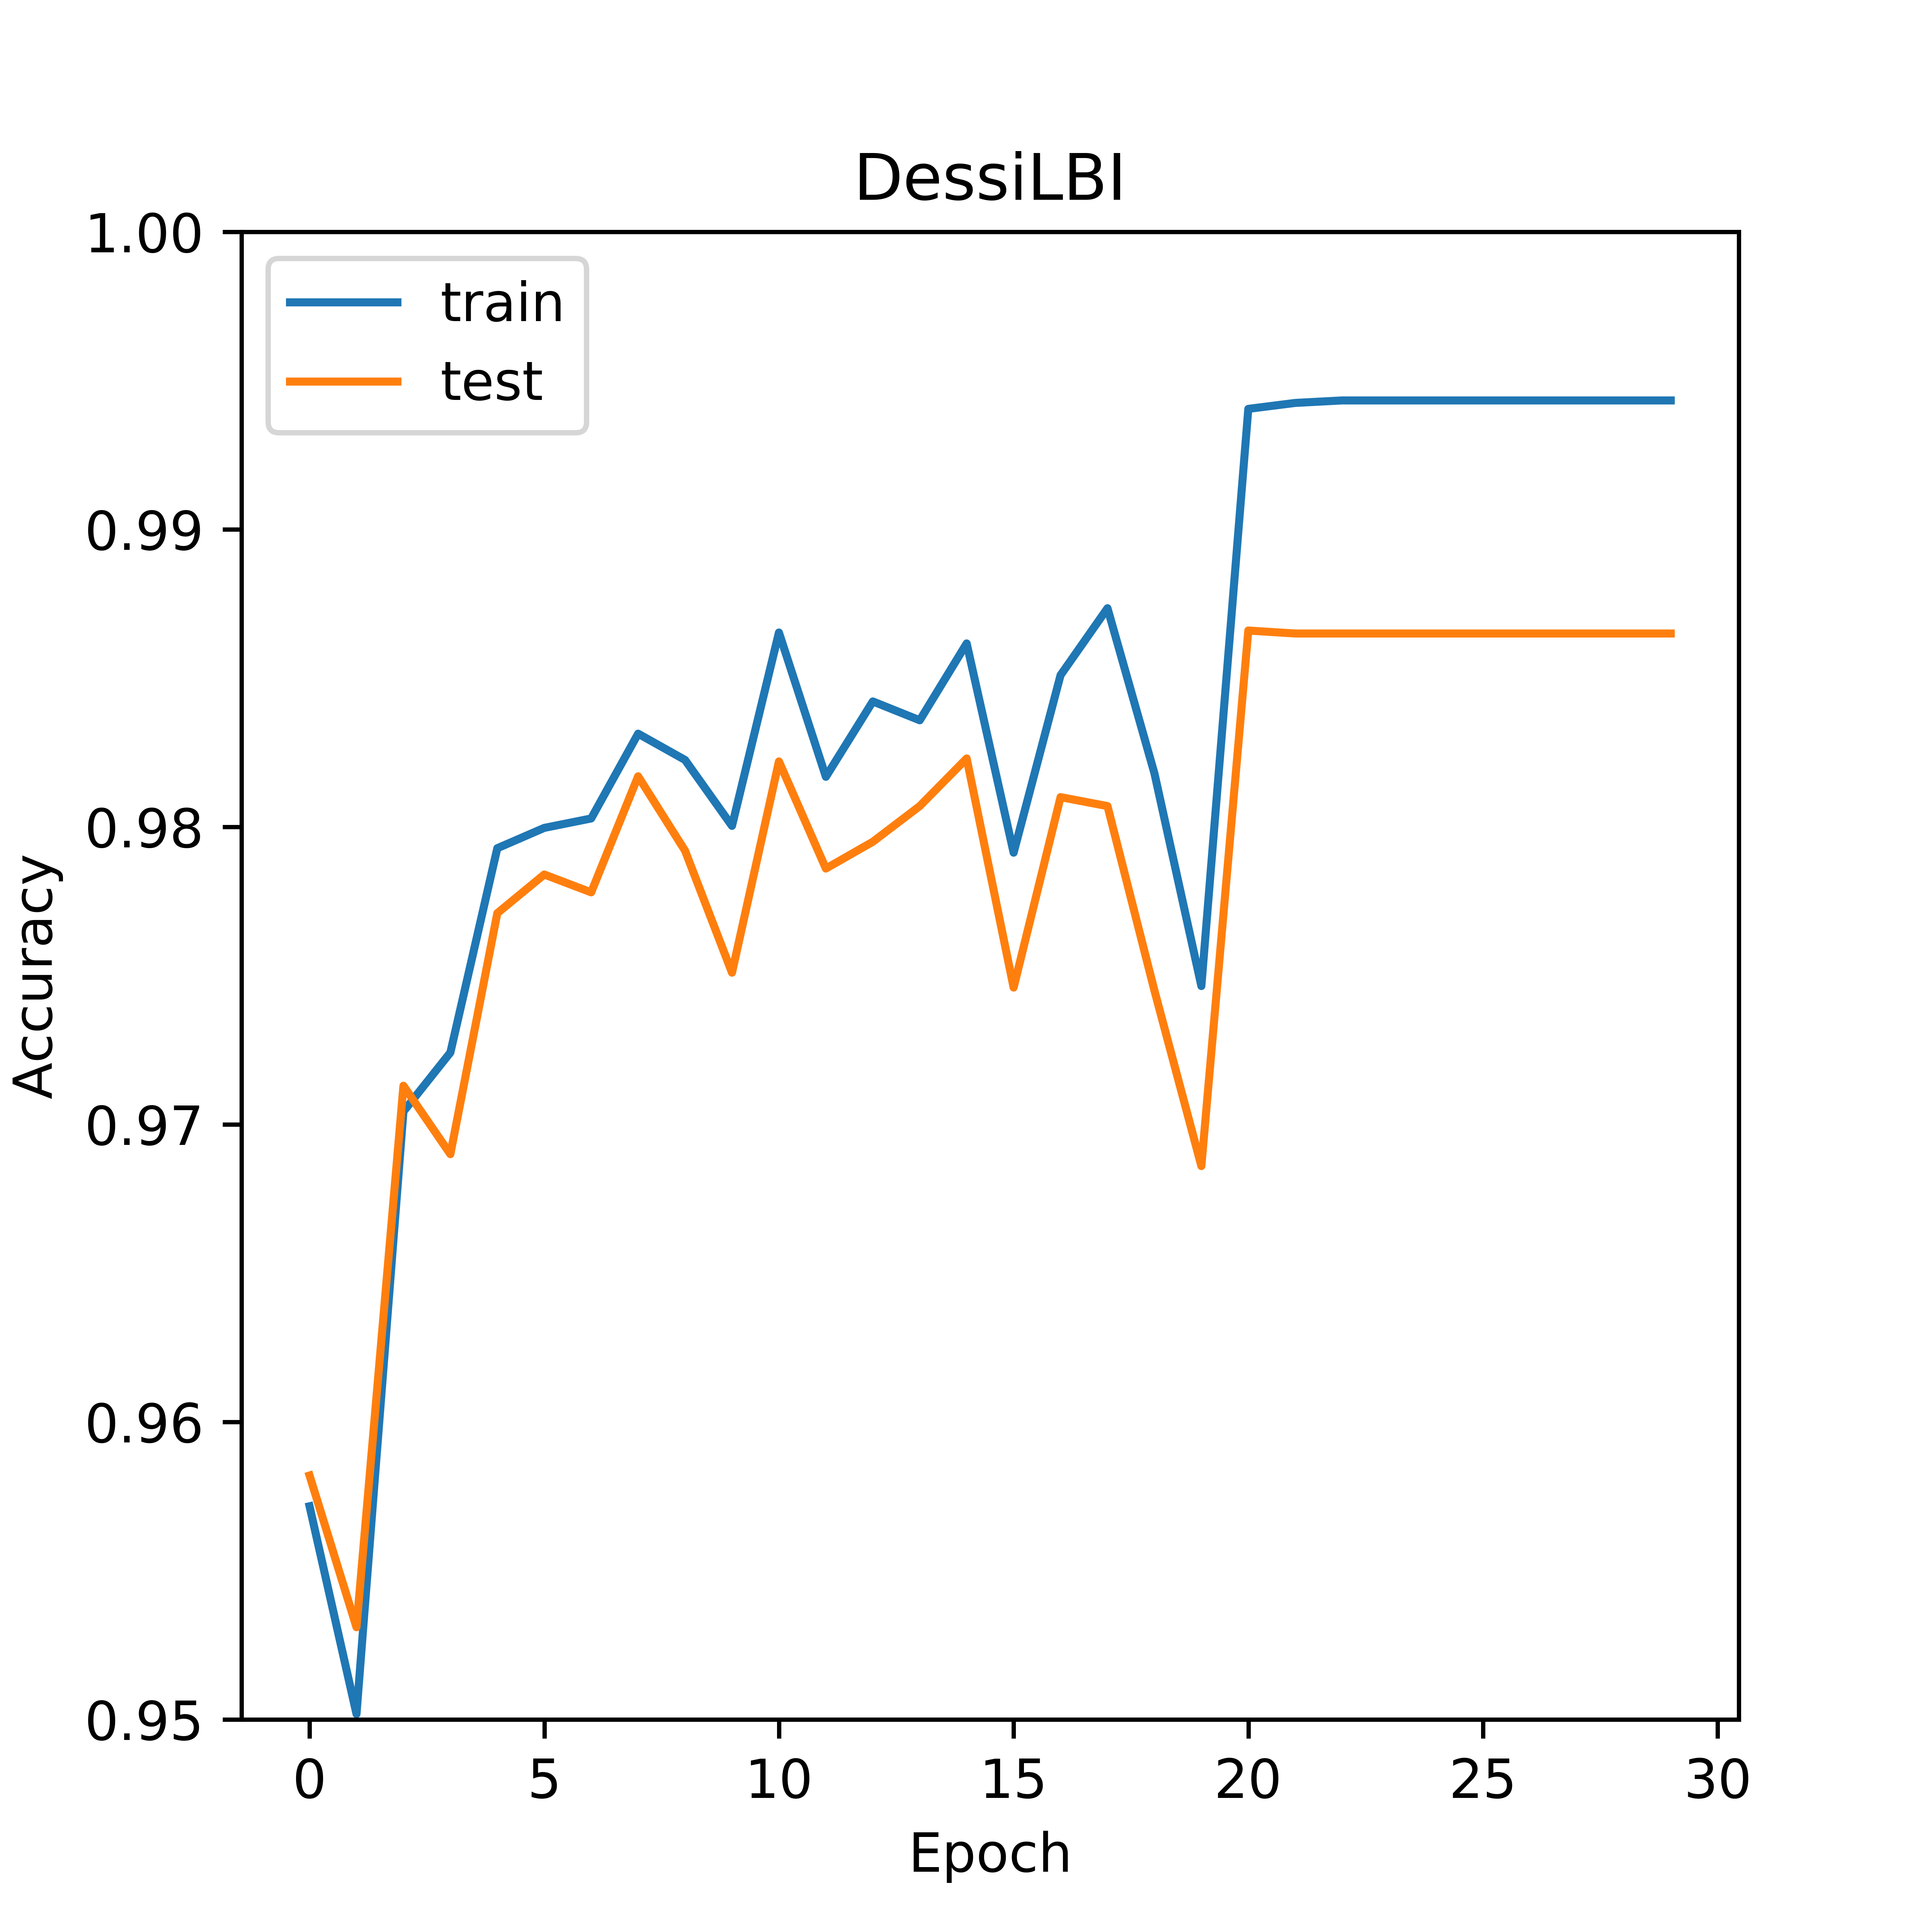
\includegraphics[width=2.5in]{./img/train-sbli.png}
	\end{minipage}
	\caption{Comparison between SGD and SLBI for LeNet on MNIST}
\end{figure}

They are of similar accuracy, while SLBI converges after about 20 epochs because of the
learning rate. Now let's prune some of the parameters on the third convolutional layer
at different rates.

\begin{table}[H]
	\begin{center}
		\begin{tabular}{ccccccc}
			\toprule
			Pruning Ratio & 0$\%$     & 10$\%$    & 20$\%$    & 40$\%$    & 60$\%$    & 80$\%$    \\
			\midrule
			Accuracy      & 98.65$\%$ & 98.65$\%$ & 98.65$\%$ & 98.64$\%$ & 98.60$\%$ & 98.30$\%$ \\
			\bottomrule
		\end{tabular}
		\caption{Accuracy of SLBI on LeNet on MNIST with different pruning ratios}
	\end{center}
\end{table}

As you can see, the pruning is successful and safe until the ratio reaches nearly 60$\%$,
which is a very high level of pruning, indicating the high degree of redundancy in model
parameters.

Here is the visualization on the third convolutional layer before and afterpruning.

\begin{figure}[H]
	\begin{minipage}[t]{0.48\textwidth}
		\centering
		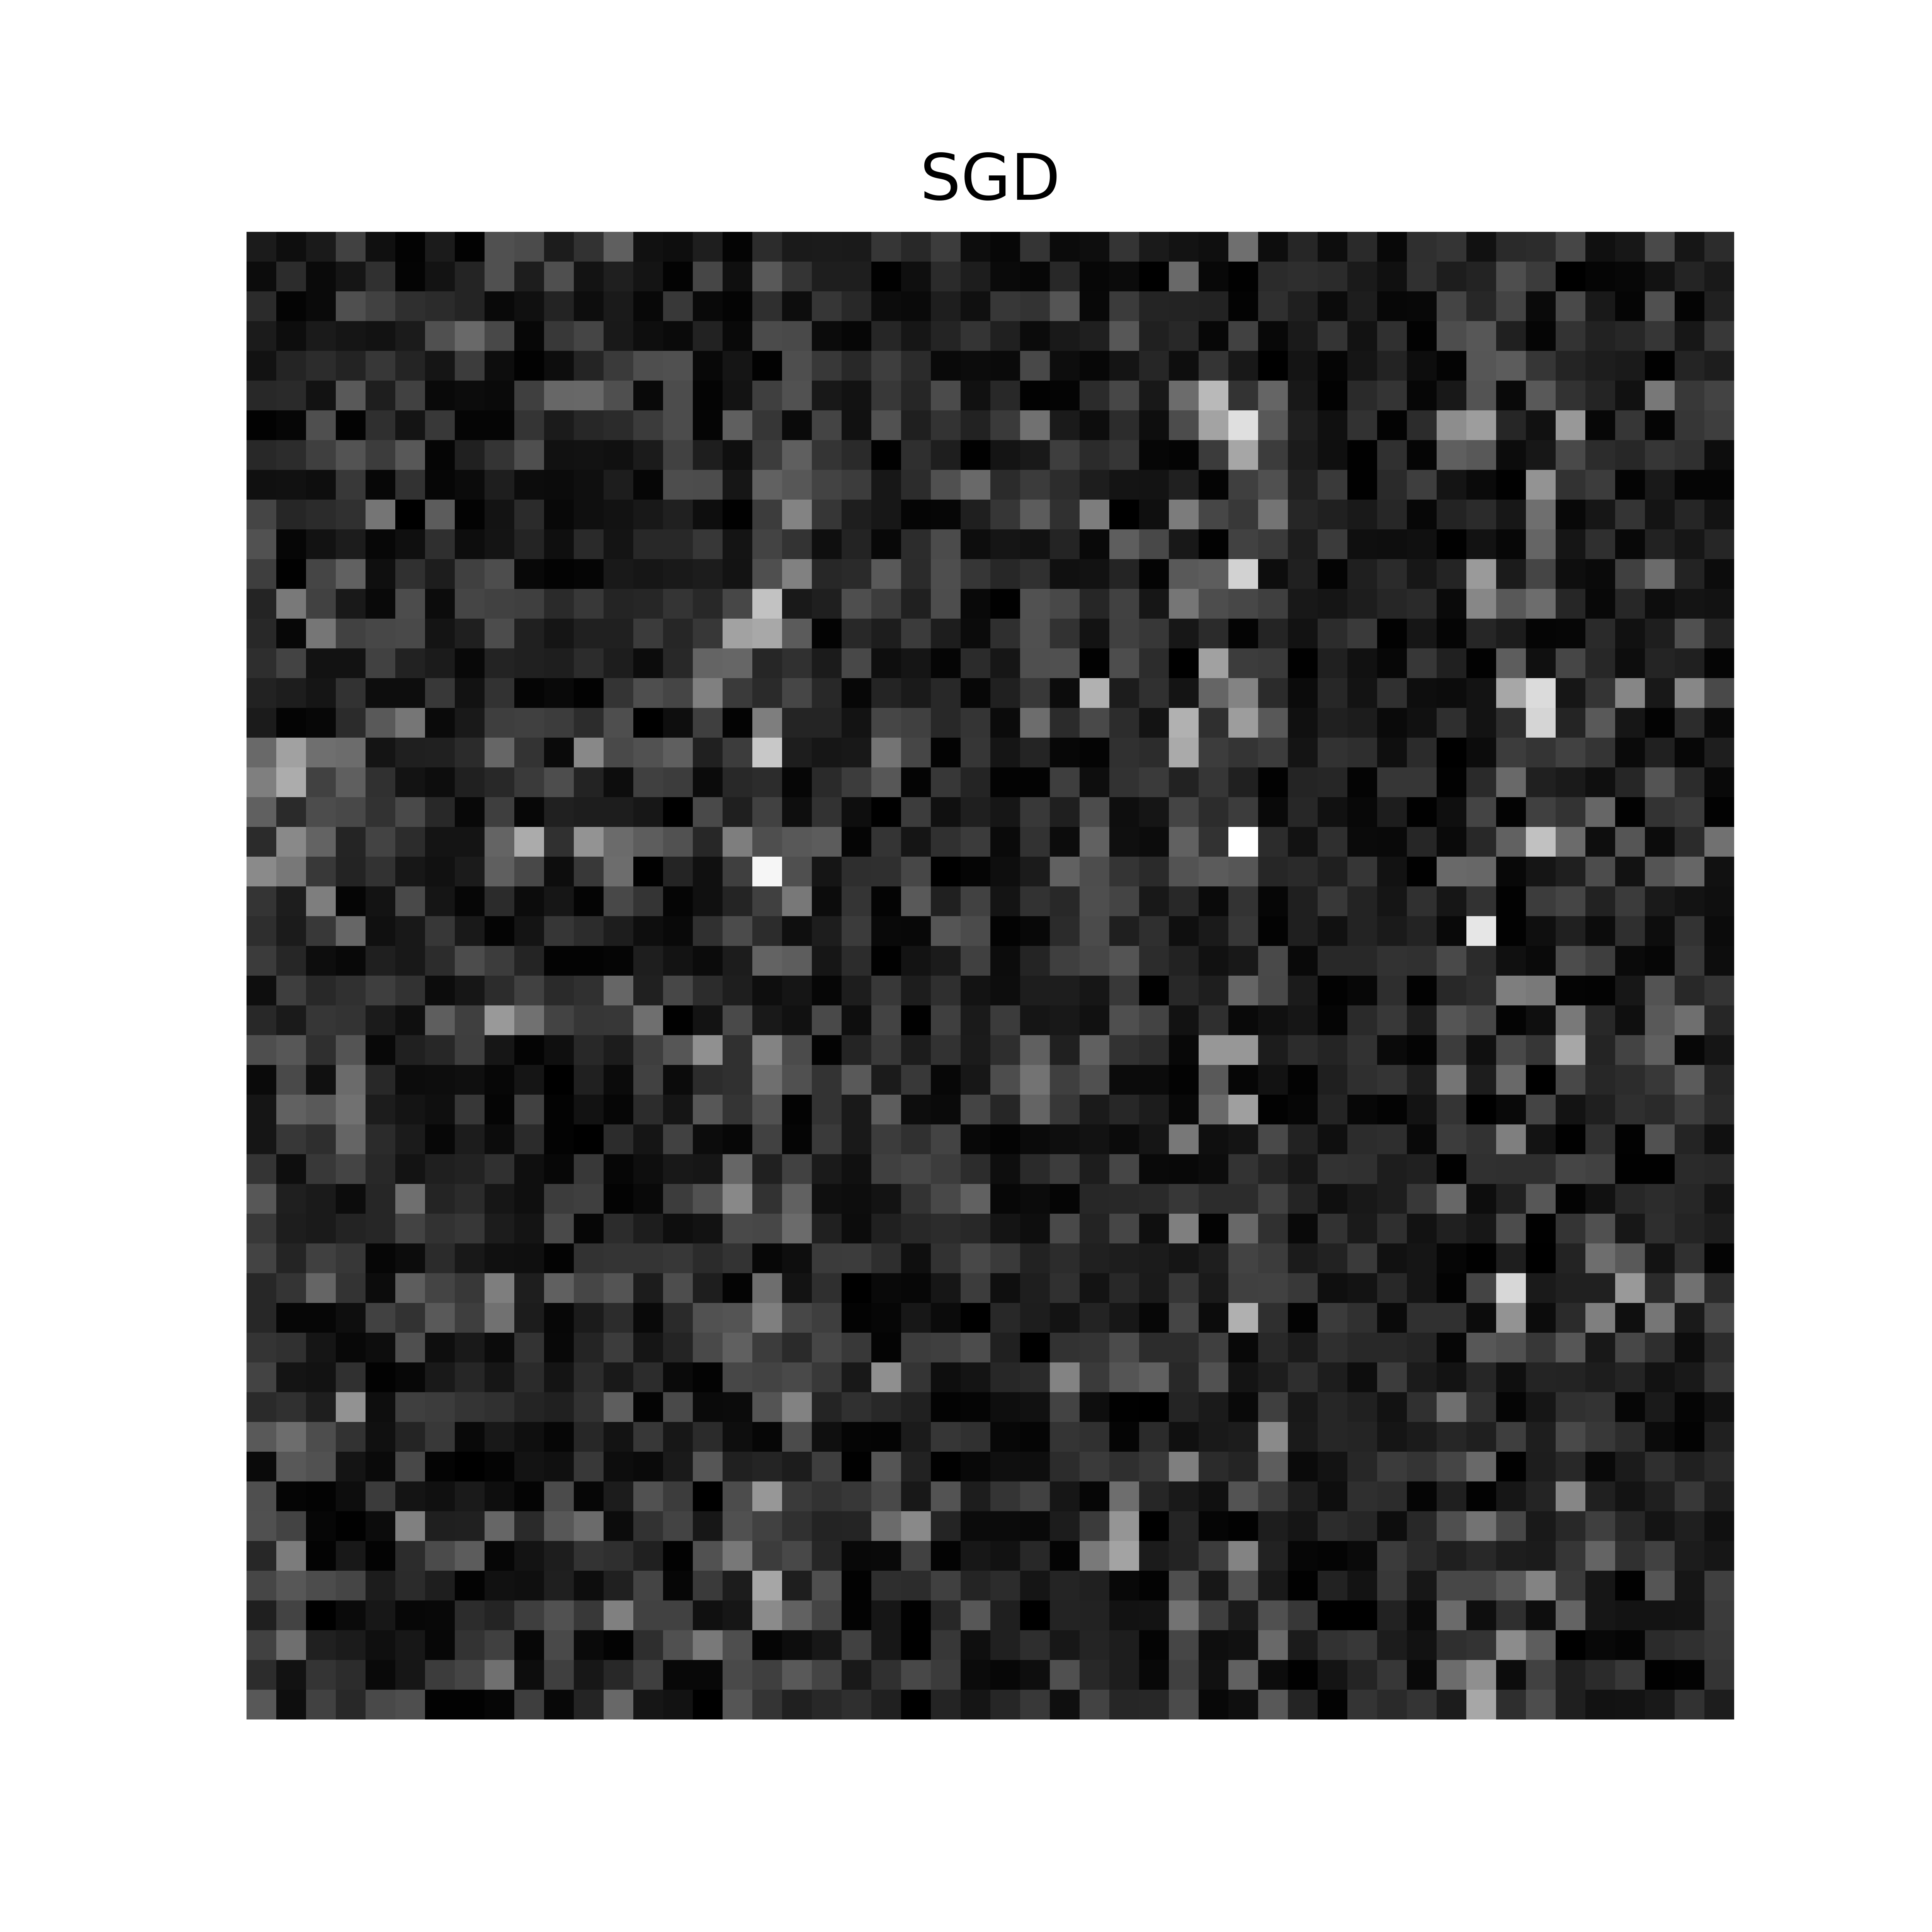
\includegraphics[width=2.5in]{./img/conv-sgd.png}
	\end{minipage}
	\begin{minipage}[t]{0.48\textwidth}
		\centering
		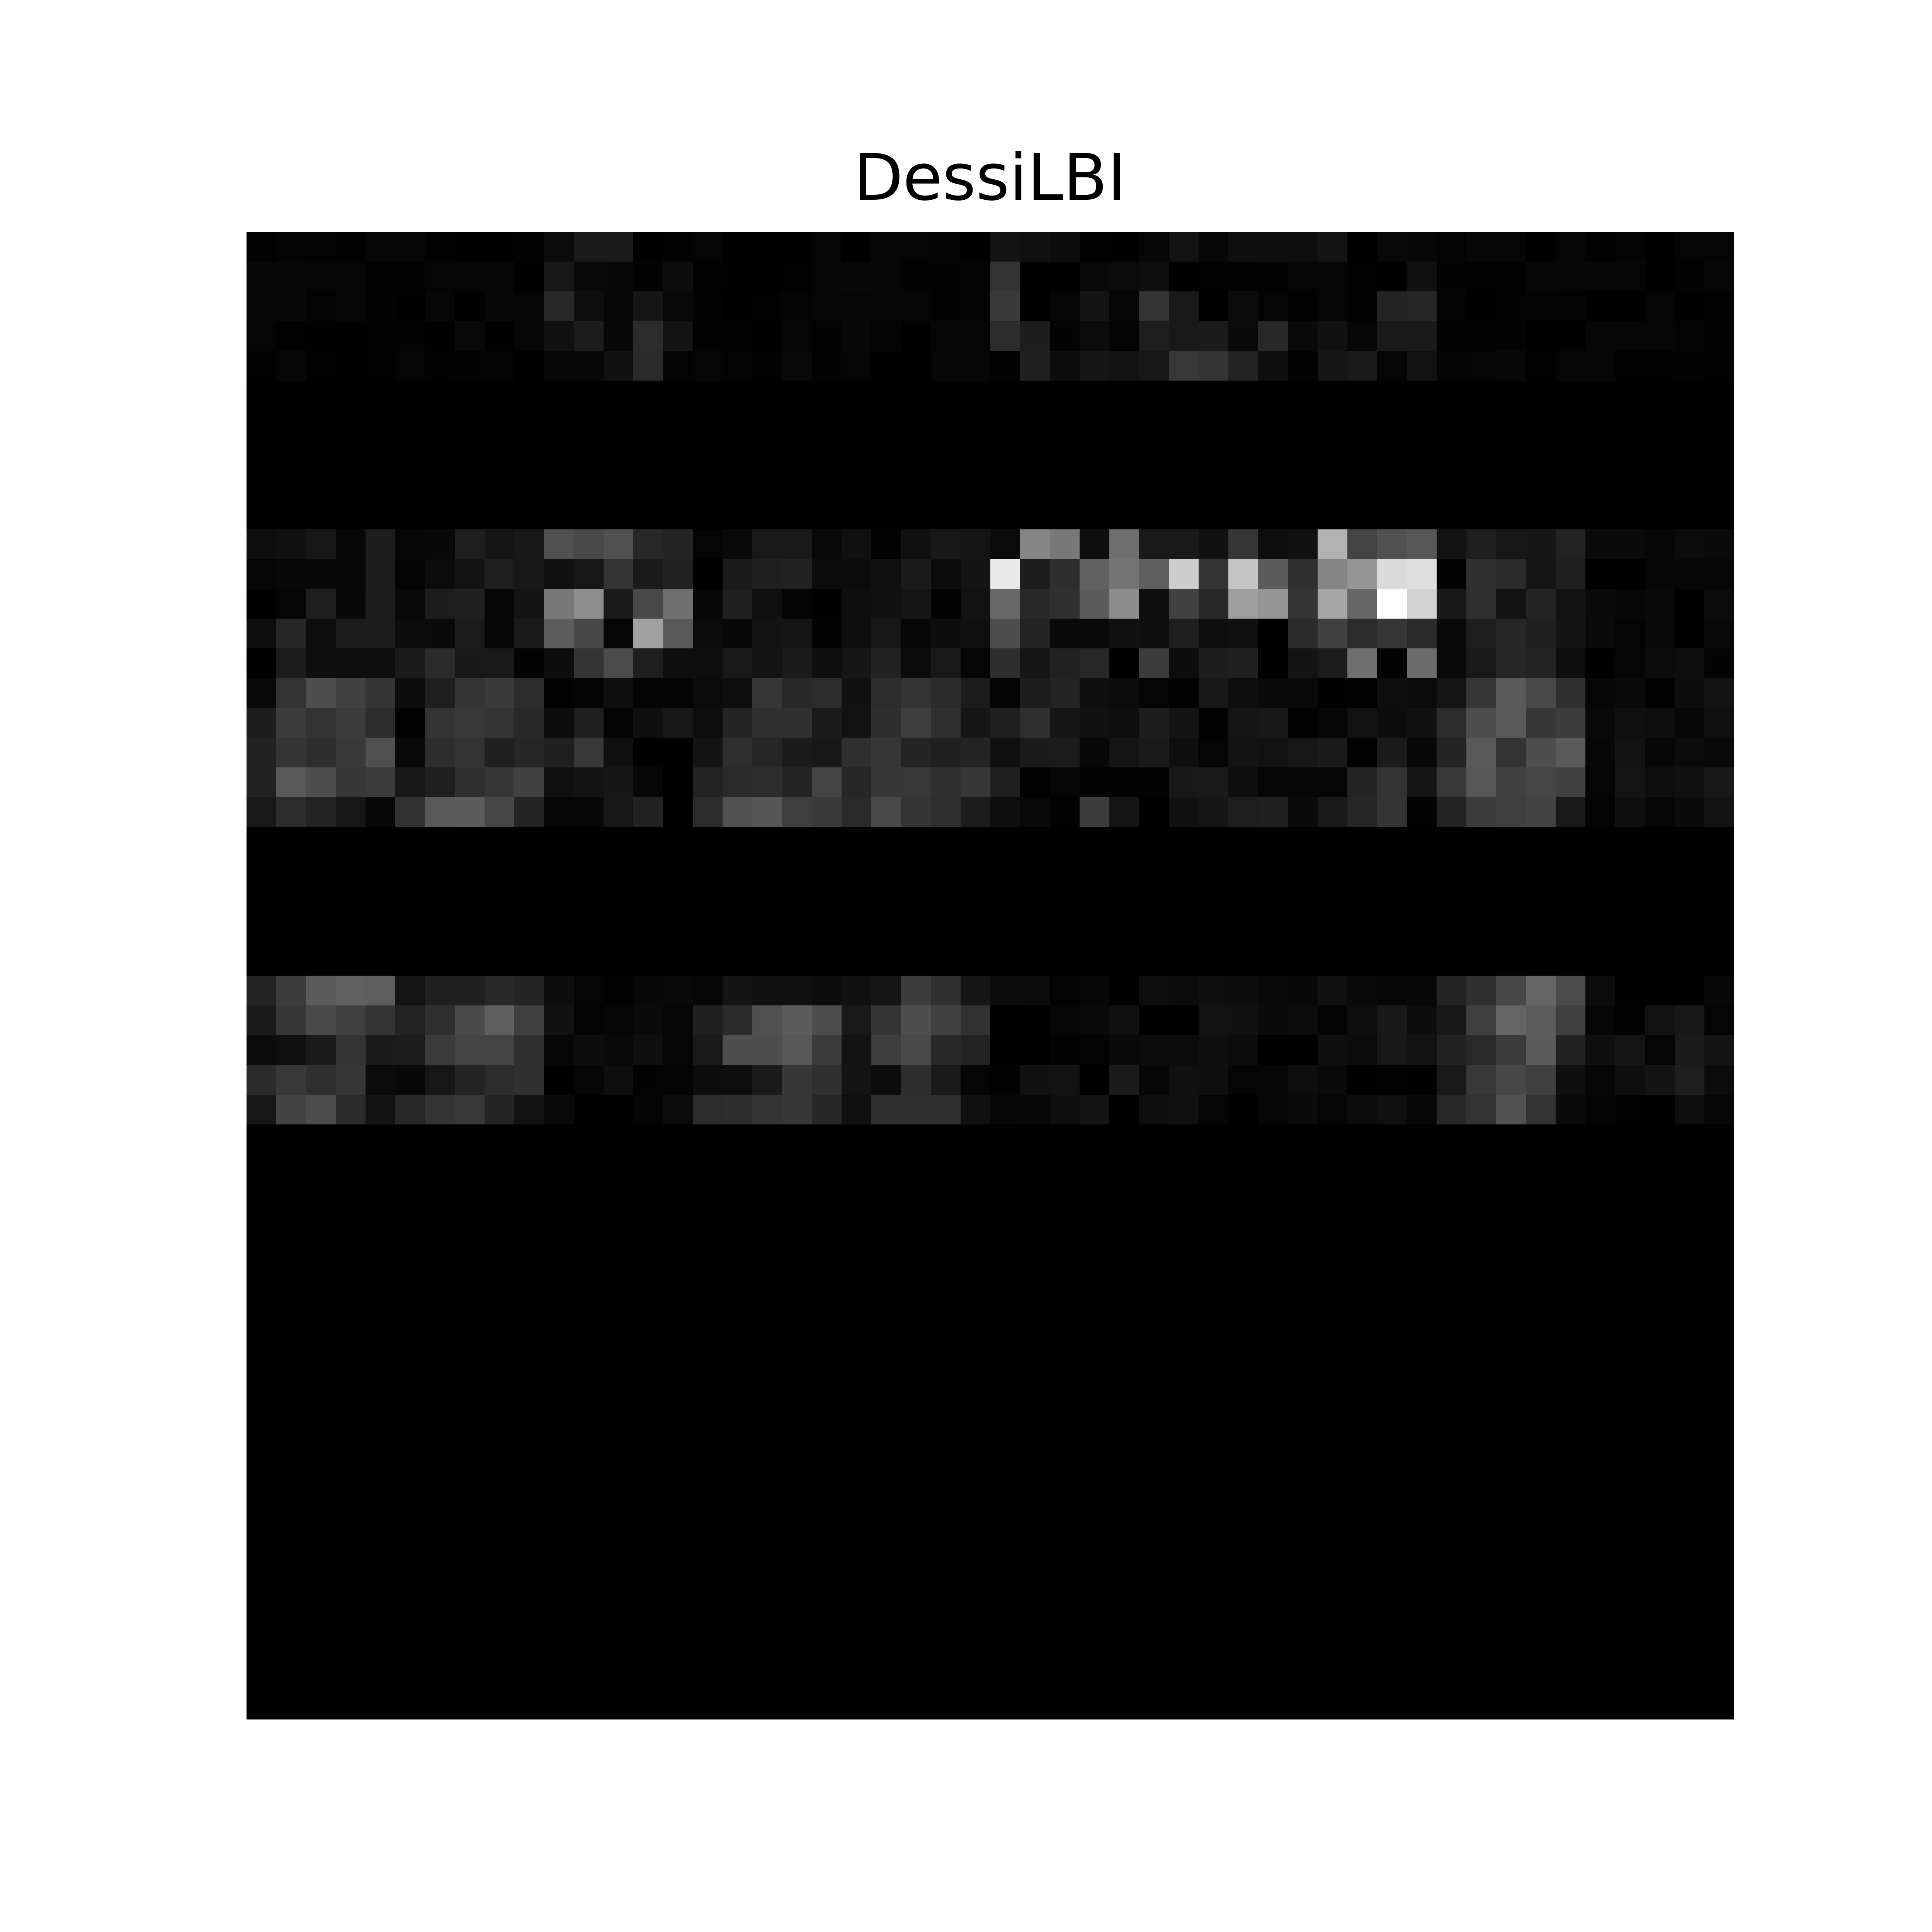
\includegraphics[width=2.5in]{./img/conv-slbi.png}
	\end{minipage}
	\caption{Visualization on 3rd Conv before and after pruning}
\end{figure}

\subsection{\textbf{Combination of SLBI and Adam}}

Referring to the official implementation of Adam, we modify the core script (step method)
of SLBI to use Adam instead of SGD. Then we train the ResNet on CIFAR-10 dataset with
both modified SLBI and Adam. The results are shown as following.

\begin{figure}[H]
	\centering
	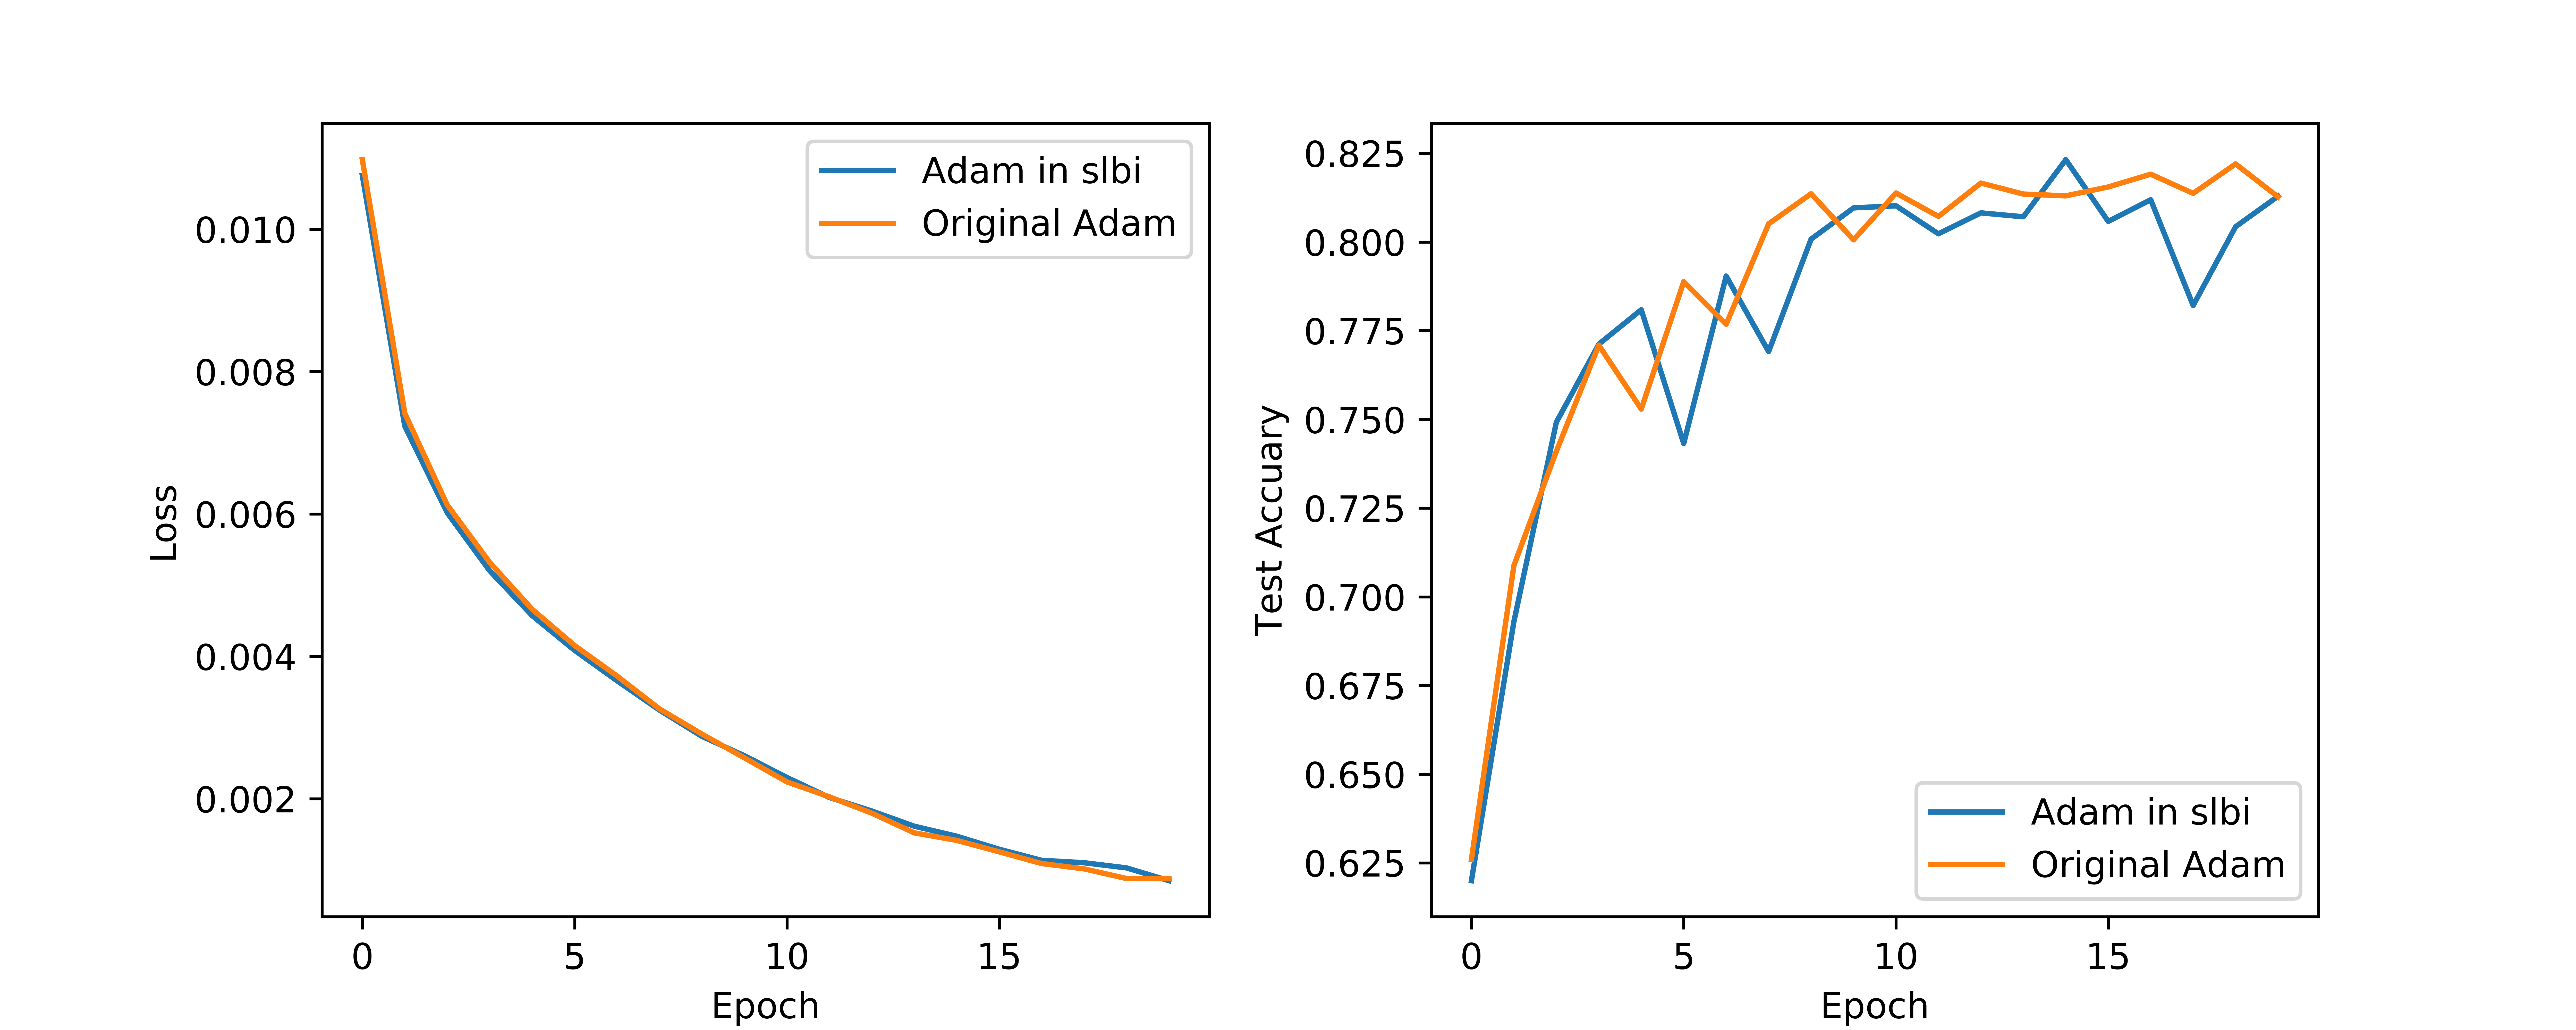
\includegraphics[width=1.0\textwidth]{./img/train-adam-slbi.png}
	\caption{Comparison between Adam and SLBI for ResNet on CIFAR-10}
\end{figure}

\begin{figure}[H]
	\centering
	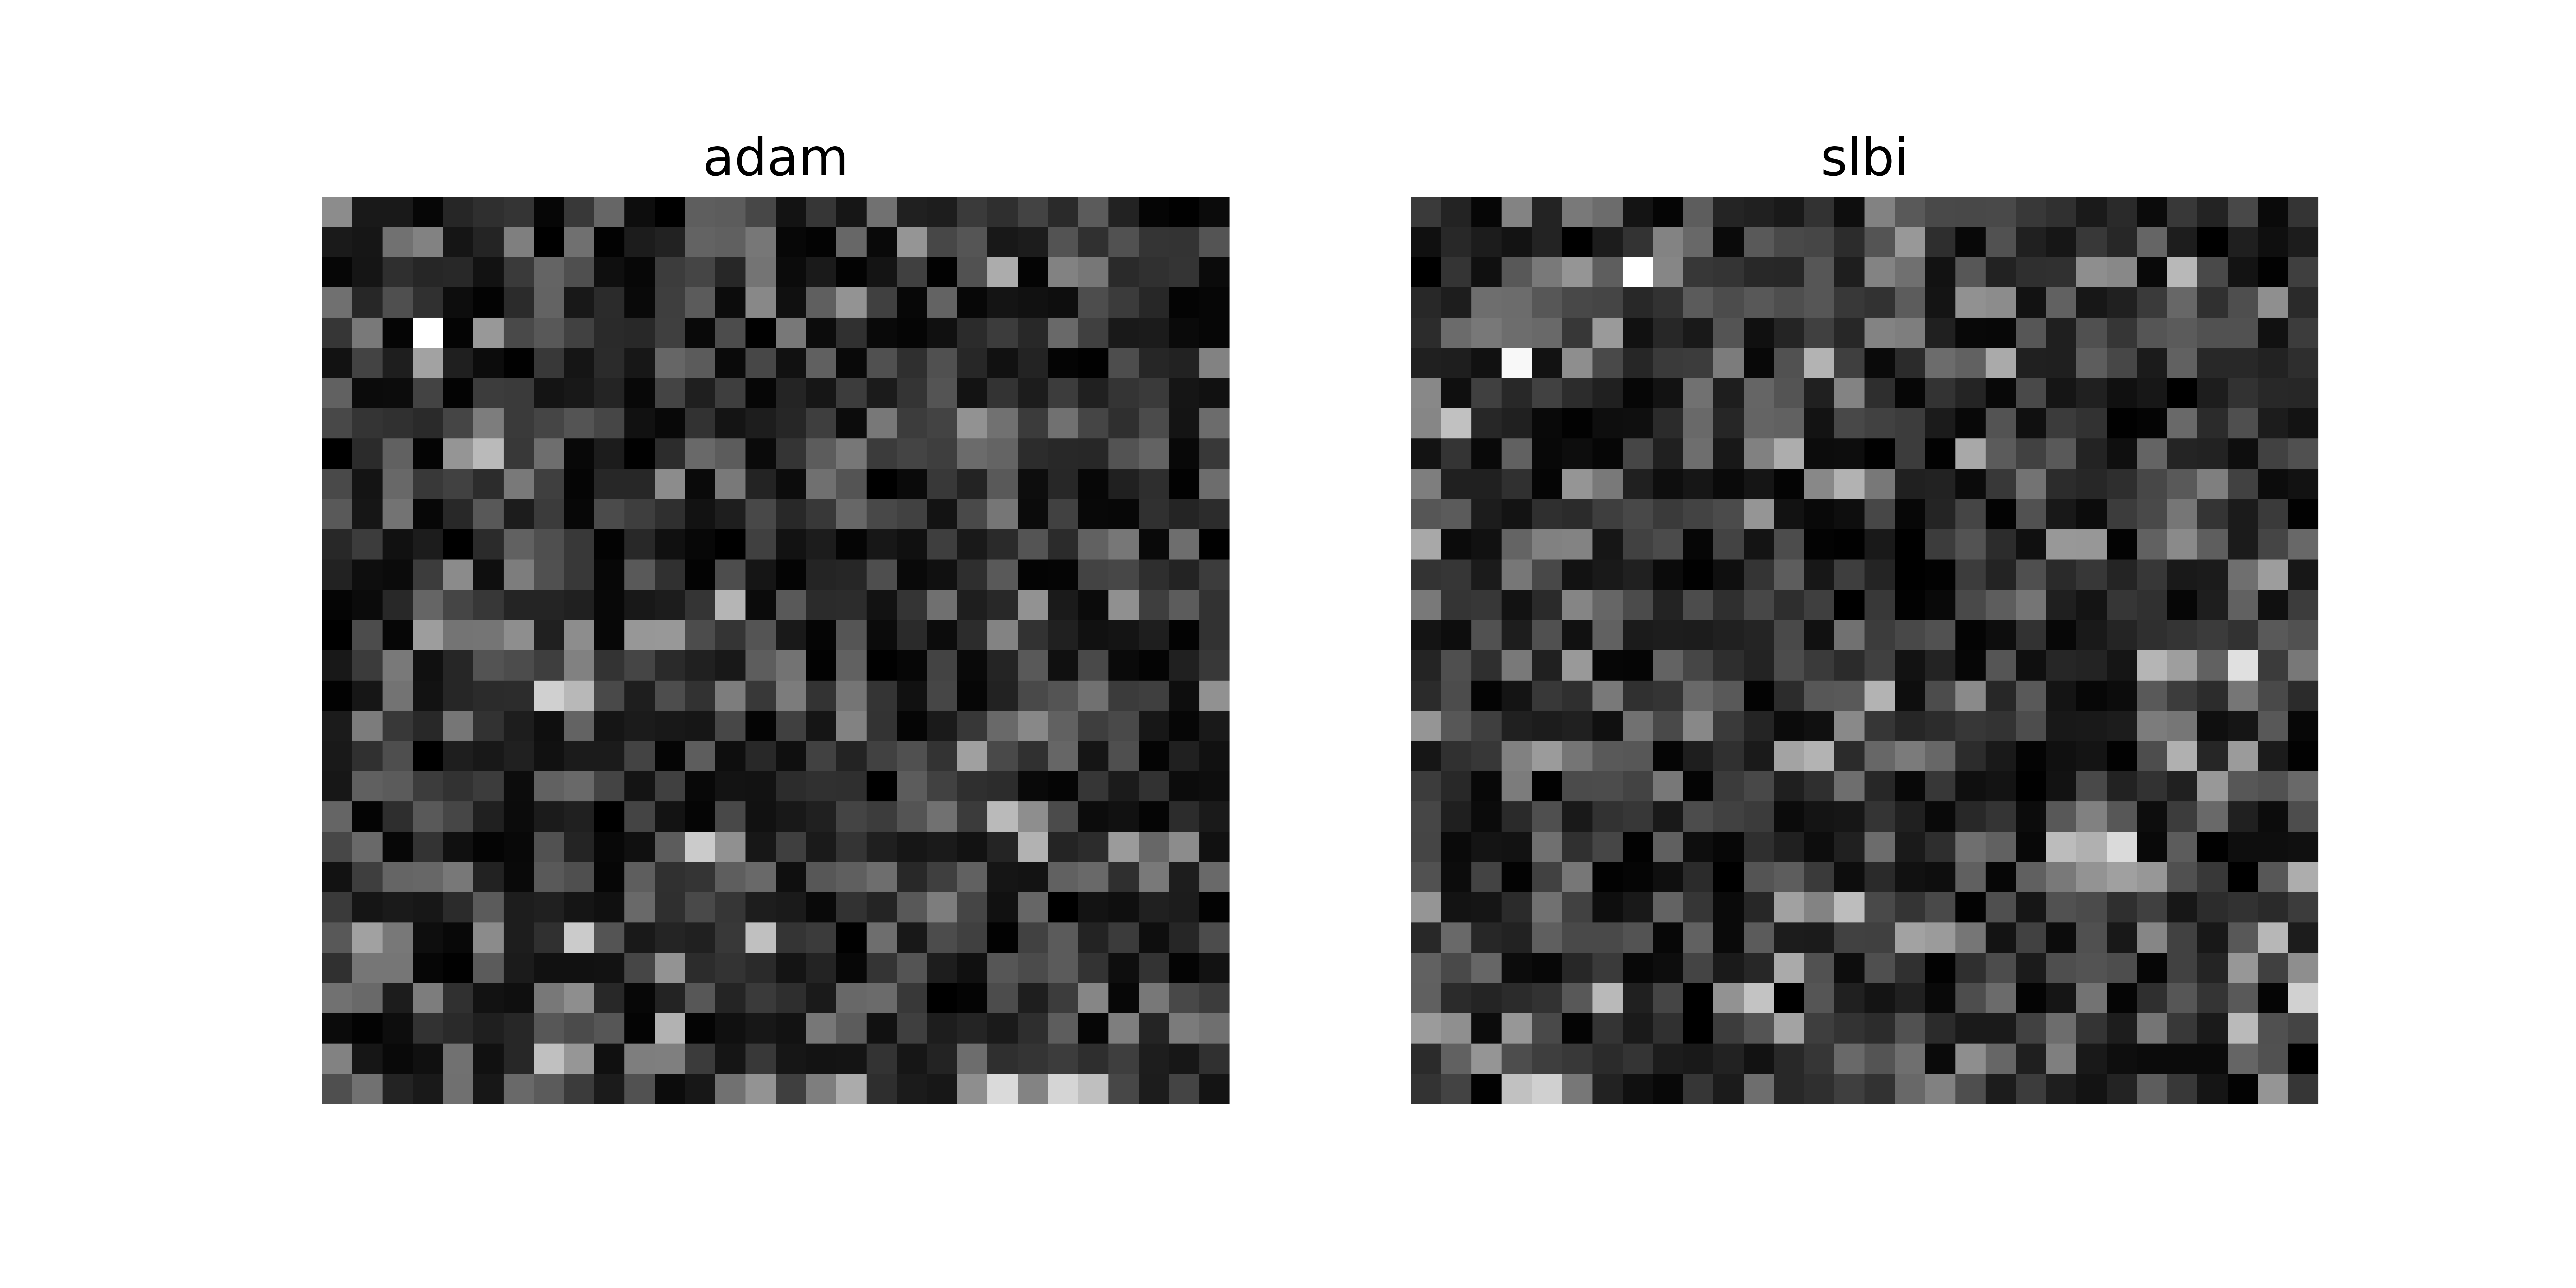
\includegraphics[width=1.0\textwidth]{./img/conv-adam-slbi.png}
	\caption{Visualization on 3rd Conv before and after pruning}
\end{figure}

There's no significant difference between them, which means the light-weight
over-parameterization in this case.

\bigskip

%----------------------------------------------------------------------------------------
%	REFERENCE LIST
%----------------------------------------------------------------------------------------

% \cite{Eureka}
% \printbibliography

%----------------------------------------------------------------------------------------

\end{document}
